%Class
\documentclass[12pt]{article}

%Package
\usepackage{multicol} 
\usepackage{graphicx}
\graphicspath{{/Users/Cho/Desktop/LaTex/}}
\DeclareGraphicsExtensions{.pdf,.png,.jpg,.jpeg}
\usepackage{listings}
\usepackage{color}
\definecolor{dkgreen}{rgb}{0,0.6,0}
\definecolor{gray}{rgb}{0.5,0.5,0.5}
\definecolor{mauve}{rgb}{0.58,0,0.82}



%Page
\usepackage{geometry}
\geometry{legalpaper, portrait}

%Header and Footer
\usepackage{fancyhdr}
\pagestyle{fancy}

%Title
\begin{document}
\begin{titlepage}
\begin{center}
\line(2,0){300}\\	
\huge{\bfseries Zikimi} \\
\textsc{\large Laptop Security Program(Java/Android)}\\[2\baselineskip]
\end{center} 

%HYU Image
\center
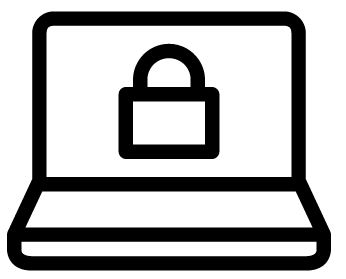
\includegraphics[width=100mm,scale=1.4]{teamlogo}
\\ [7\baselineskip]


%KunShik(Top Left) 

\begin{multicols}{3} \noindent 
\textsc {\noindent KunShik Cho\\ 
Information System in HYU \\
 2011004705 \\ 
 william109@naver.com}\\[1\baselineskip]
%GiChang(Bottom Left)
\textsc{Gichang Shin \\
 Information System in HYU 
 \\ 2011004501 \\ 
 skc0413@naver.com}\\[1\baselineskip]
%DongHyeuk (Top Right)			
\textsc{DongHyeuk Lim \\
Information System in HYU \\
2011027074 \\
capdh@naver.com} \\[1\baselineskip]
\end{multicols}
\end{titlepage}



%Table of Contents
\tableofcontents
\pagenumbering{roman}
\cleardoublepage
%\addcontentsline{toc}{section}{\numberline{}Test}



%Abstract
\pagenumbering{arabic}
\setcounter{page}{1}
\section{Abstract}

If you set up our program into your laptop computer and connect with smart phone application, you can confirm laptop computer camera screen. And our program can do other things. If there is Attempts for theft, you can warn to theft. Also you can record camera screen and receive status report. And last, if your laptop computer is stolen, you can lock your laptop computer.\\





%Introduction
\section{Introduction}

Many people lose their laptop computer. In the cafe and library, Many people feel anxiety but they just vacate for a while leaving laptop computer. Because there is no other choice. But there are many burglaries in the cafe and library. And you can see many articles about this accident. As an example, in the Hanyang University, A student lose his laptop in the library. But if you can know your laptop computer’s situation in real time and can give warning to thief, it will be very helpful to many laptop computer’s owner. Our project begins at here. If you set up our program into your laptop computer and connect with smart phone application, you can confirm laptop computer camera screen. In addition, you can protect your laptop computer by giving warning to thief. Also after Laptop computer stolen, you can use tracking and locking function by our program. Through such a procedure, laptop computer’s owner can vacate for a while, feeling relieved. 

\section{Requirements}


\subsection{Basic Function}
- Real time Streaming\\
- Real time Streaming ON/OFF button\\
- Log-in page\\
- Password page in entire program ON/OFF function\\
- Small icon function(Hiding function)\\

\subsection{Warning System}
- Remote-control alarm by pressing the button\\
- Warning page come out by pressing the button\\
- Warning message changing function\\
- Various types of alarm(Sound changing function)\\
- Auto warning ON/OFF\\
- Alarming when someone releases the charger\\
- Alarming when someone releases USB\\
- Alarm duration set-up function\\


\subsection{Recording System}
- Motion recording\\
- Motion recording Auto/Manual conversiong function\\
- Motion photographing function\\
- Manual photographing function\\

\subsection{Situation Reporting System}
- Sending situation notification push-message when motions caught\\
- Sending notification message when the battery ran out\\
- Sending push-message when the auto warning activated\\
- ON/OFF buttons of each situation reporting functions\\
- Setting counts of messages in each situation reporting functions\\

\subsection{Lock System}
- Manual remote-control lock function\\
- Locking when auto warning activated\\
- Auto Warning Lock ON/OFF button\\
- Releasing Lock by using the app\\

%Table
\section{Role Assignment}
\begin{table}[htb]
\centering
\caption[Role Assignment]{Role Assignment}
\begin{tabular}{|c|c|p{6cm}|}
\hline
\textbf{Roles}& \textbf{Name} & \textbf{Task Description and Etc.}\\ \hline

User & Shin & -Using the program\par
-beta testing\par
-writing review and suggestions
\\ \hline

Customer & Shin & -Using the program\par
-beta testing\par
-writing review and suggestions\\ \hline

Software Developer & Lim & -Coding the program\par(C-Sharp/android)\par
-Alpha testing\par
-Maintenance.
\\ \hline

Developer manager & Cho & -Documentation\par
-Supervising developer\par
-Promoting the program.
\\ \hline

\end{tabular}
\end{table}


%Development Environment
%Section
\section{Development Environment}
%Subsection 1
\subsection {Choice of software development platform} 

%Subsubsection 1
\subsubsection{Which platform and why?}
We will use Windows, Android and Web. We considered that most of normal people use these platforms. So, the main reason why we choose these is the market share.

\begin{itemize}
%
\item\textbf{Windows}\\ 
\\As you can see in this picture, in January 2016, almost 90 percentages of Worldwide OS market share is Windows. Also, all of our team members' OS are Windows too..\\[2\baselineskip]
%
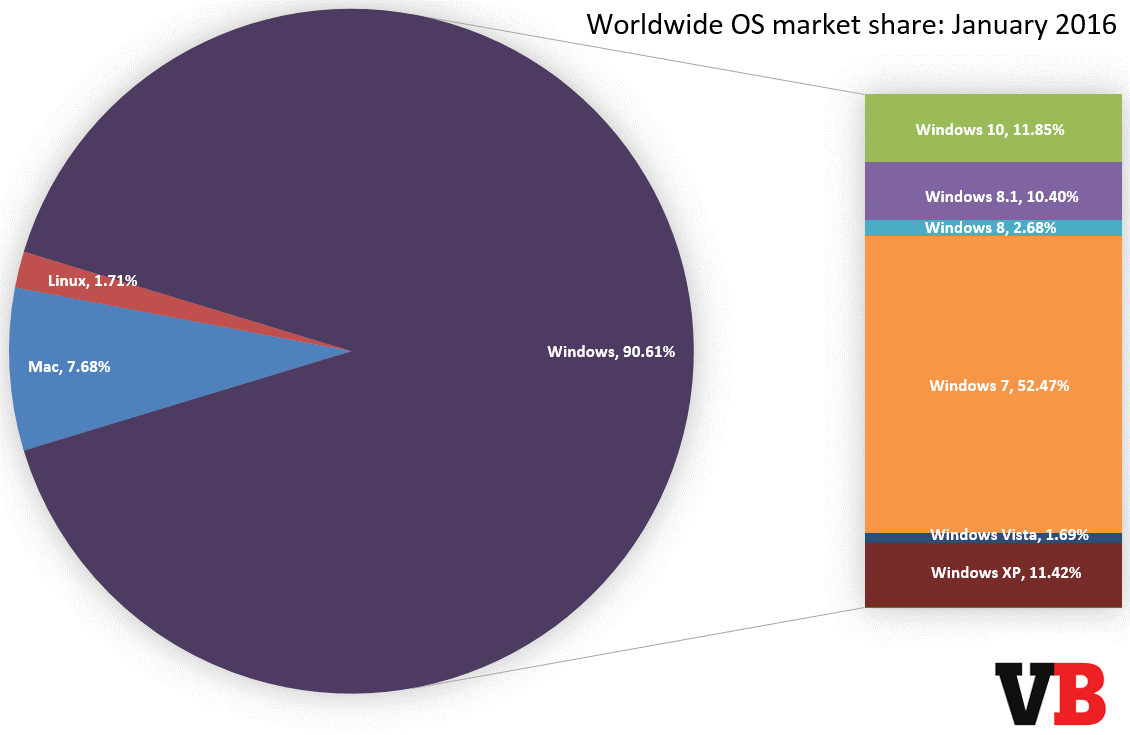
\includegraphics[width=140mm,scale=2]{windowsgraph}
%

\item\textbf{Android}\\
\\This is the market share of smart phone OS. Android's market share is overwhelmingly higher than the others. Also, our team members, DongHyeok and KunShik use Android version Lollipop and KitKat.\\
Android has more reasons. Android enables developers to build applications in JAVA language and provides a run-time library that can drive the compiled byte code. It also provides a variety of tools and API required to develop an application through the Android Software Development Kit (SDK). Since we will use JAVA, this is the significant advantage for us. In addition, Android has an active community of developers who use the Android Open Source Project (AOSP) source code to develop and distribute their own modified versions of the operating system.
 \\ 

\begin{center} 
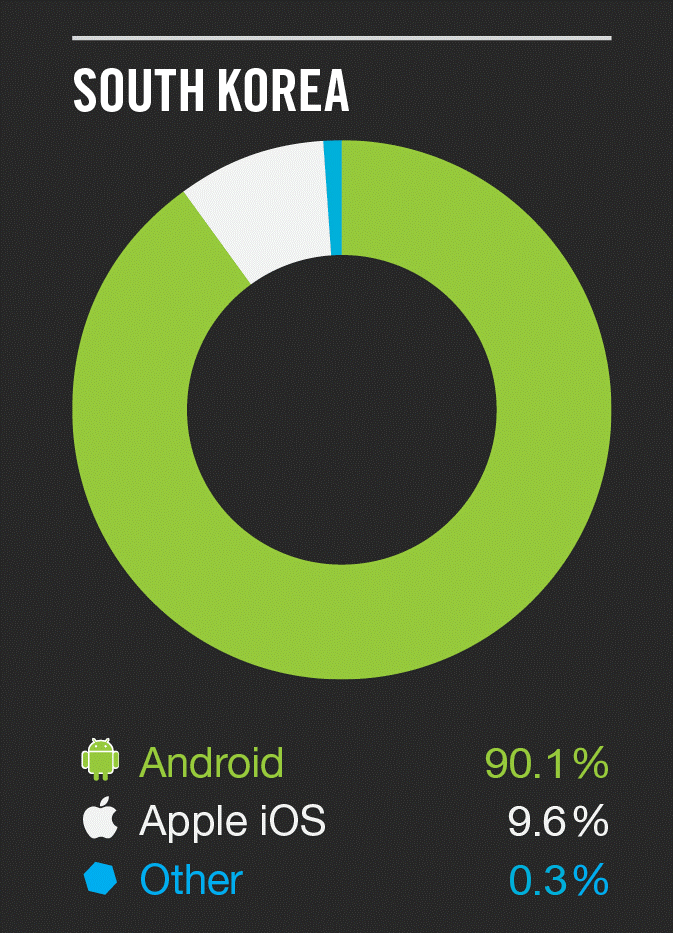
\includegraphics[width=100mm,scale=1.5]{androidgraph}
\end{center}
%
\item\textbf{Web}\\
\\To build Zikimi's Login and Logout functions, we need Web to manage users who use our program. We are trying to use JAVA language, so the below is for example.\\
Realizing Loging function briefly in java code.\\
try {\\
MemberManager.getInstance().login(\\
request.getParameter("id"),request.getParameter("password"));\\
// the part of acting code after normal Login\\
} catch (NoSuchMemberException ex) {\\
// if there is no applied user to ID\\
} catch (InvalidPasswordException ex) {\\
// wrong password\\
} catch (ServiceNotActiveException ex) {\\
// exceptions in service problems like database connection\\
}
\\

\end{itemize}

%Subsubsection 2
\subsubsection{Which programming language and why?}
 We will use C-Sharp because C-Sharp has a great WebView. We will use Web view. So this is huge advantage to our team. And C-Sharp has a lot of advantages. It is automatic garbage collection So we can easily manage memory. And It don’t need pointer anymore. We are student so we have very difficulty in C’s pointer. \\
 Actually We are concerned about Java and C-Sharp. But there are many advantages in C-Sharp over java. Usually it is much more efficient than java and runs faster. And It has more primitive type(value type), including unsigned numeric types. We also can se more clean events management(using delegates)\\


%Subsubsection 3
\subsubsection{Cost estimation}
\begin{center} 
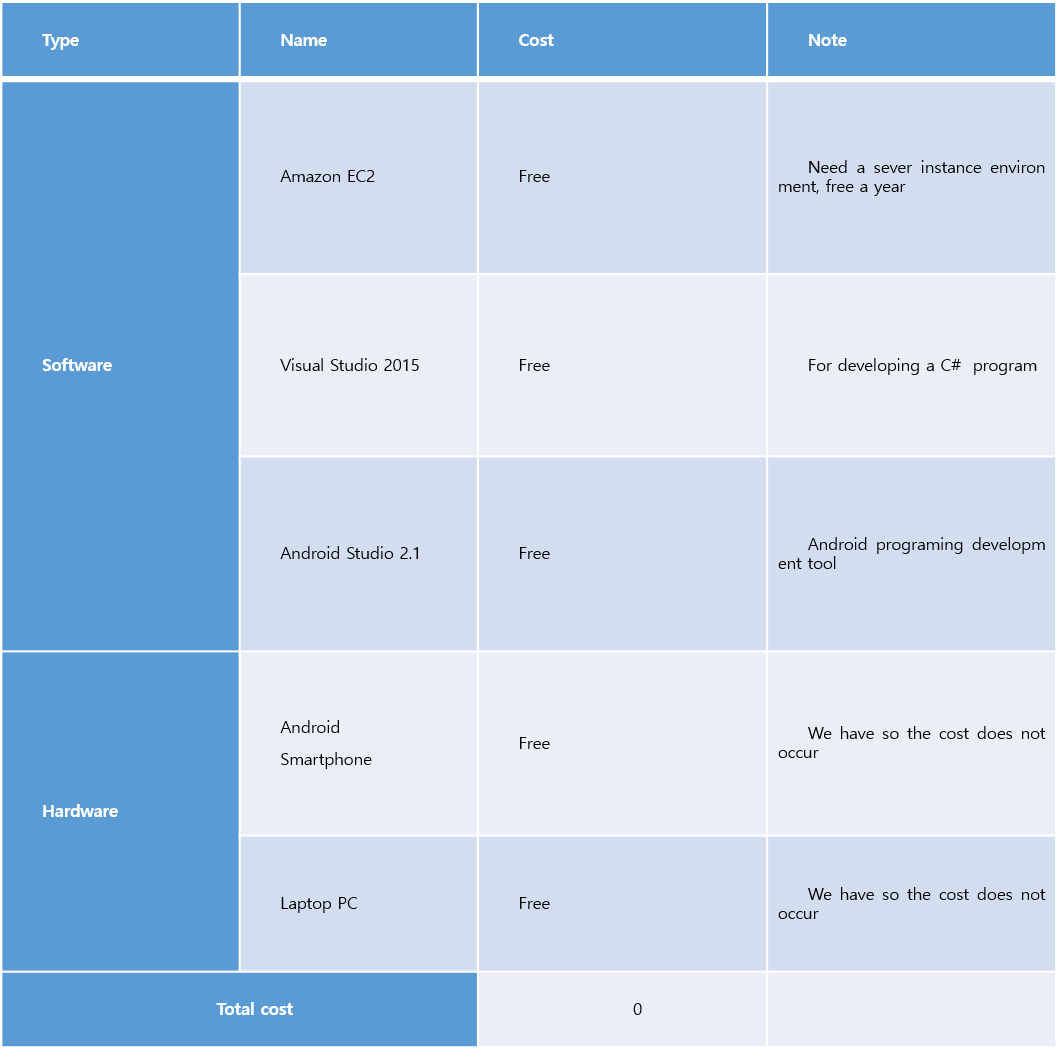
\includegraphics[width=150mm,scale=2.2]{cost}
\end{center}

%Subsubsection 4
\subsubsection{Clear information of  our development environment}
\begin{enumerate}
\item GiChang\\
\\LG gram14(LG14Z95)\\
CPU - Intel(R) Core(TM) i7-5500 CPU @ 2.40GHz\\
RAM - 8.00GB\\
OS - Windows 7 (64bit)\\
Android studio\\
Android version Lolipop\\

\item KunShik\\
\\LG gram14(LG14Z95)\\
CPU - Intel(R) Core(TM) i7-5500 CPU @ 2.40GHz\\
RAM - 8.00GB\\
OS - Windows 7 (64bit)\\
Java version 8\\
Android studio \\
Android version Lolipop\\

\item DongHyeuk\\
\\Hansung forcerecon U45X-3557\\
OS - Windows 7 (64bit)\\
Cpu - Intel Core I5-5200U CPu 2.20GHz\\
Ram - 4.00GB\\
SSD – 120g\\
Java version 8\\
Android studio \\
Android version Lolipop
\\

\end{enumerate}

%Subsubsection 5
\subsubsection{Using any commercial cloud platform}
We will use Amazon’s EC2. Because we need Login/Logout function. We will use PHP to operate the Loing/Logout function. So we will stack up php application on the Amazon’s EC2.

\subsection{Software in use}
\begin{enumerate}
\item There is code that laptop computer’s camera screen sending to the android machine. It uses JMF API.\\ In this project, Work flow is myPlayer - FrameGrabbingControl fgc - fgc.grabFrame() - Buffer buffer - BufferToImage btoi
- Image image - Image photo.

\item Stream Media Player - Stream Media Player is an application that provides an ability to play video from web cameras, watch Internet TV, and play locally stored files. Internet Radio widget.
\item Visited links are saved in history. The player also contains links DB updated from the server.\\
(https://play.google.com/store/apps/details?id=com.psa.android.mediahl=en)\\
SoftKeep 1.4 - http://www.softhearts.co.kr/31\\
Lalarm 5.7 - http://www.lalarm.com\\
DroidCam - http://www.dev47apps.com/droidcam/\\
CameraFi
\item Use case - AVM (Around View Monitor) System\\
\begin{center} 
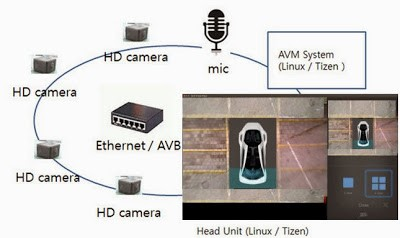
\includegraphics[width=120mm,scale=2]{avm}
\end{center}
\end{enumerate}

\subsection{Task Distribution}

\begin{enumerate}
\item GiChang Shin\\
\\Amazon Web Service EC2 - Web server :\\
It uses the EC2 Cloud computing service provided by Amazon Web Service to the Web server. Using the EC2 computer to build a Web server environment.\\
\\Web RTC API :\\
Web RTC (Web Real - Time Communication) is an API that is designed to communicate with each other without the help of a web browser plug-in between. The draft presented at the W3C, which can be used as voice calls, video calls, P2P file sharing. The Media streaming (Voice, Video), Data transfer function between the user which is provided by Web RTC will implement real-time video communication and message transmission between Laptop and Android Smart-phone. Through the Web server built into EC2, we will use Web RTC API.\\
\item KunShik Cho\\
\\Web View :\\
 WebView contain streaming web that used webrtc api. And it has two methods. First thing is setNumber(). This method get special number from user. This number will be used at android to see the laptop’s camera screen. Second thing is Show(). This method is used at show the contents of streaming screen.\\
\\Button : \\
Button is used to resize the C-Sharp program screen at minimum. To hide the laptop’s camera screen at laptop. User must use this button to hide their camera screen. \\
\item DongHyeuk Lim\\
\\Main Activity : \\
It has three methods. First thing is soundAlert. User can see the thieves by android application. So if user see the thieves, user can push the soundAlert button to ring the alert bell at the laptop. Second thing is getNumber. User can get number from laptop by this method. Third thing is join. User can connect to the laptop by this method.\\
\\Web View : \\
WebView contain one method that is Show(). This method is used at show the contents of streaming screen from laptop.\\
\item All Together\\
\\Actually, our team members participates every tasks without reference to the task distribution\\
Also, latex and documentation tasks have been done together.\\
\end{enumerate}




%subsection 3

\newpage \section{Specification}

%subsubsection 3

\subsection{Basic Function}

%Subsubsection 1
\subsubsection{Streaming}
\begin{center} 
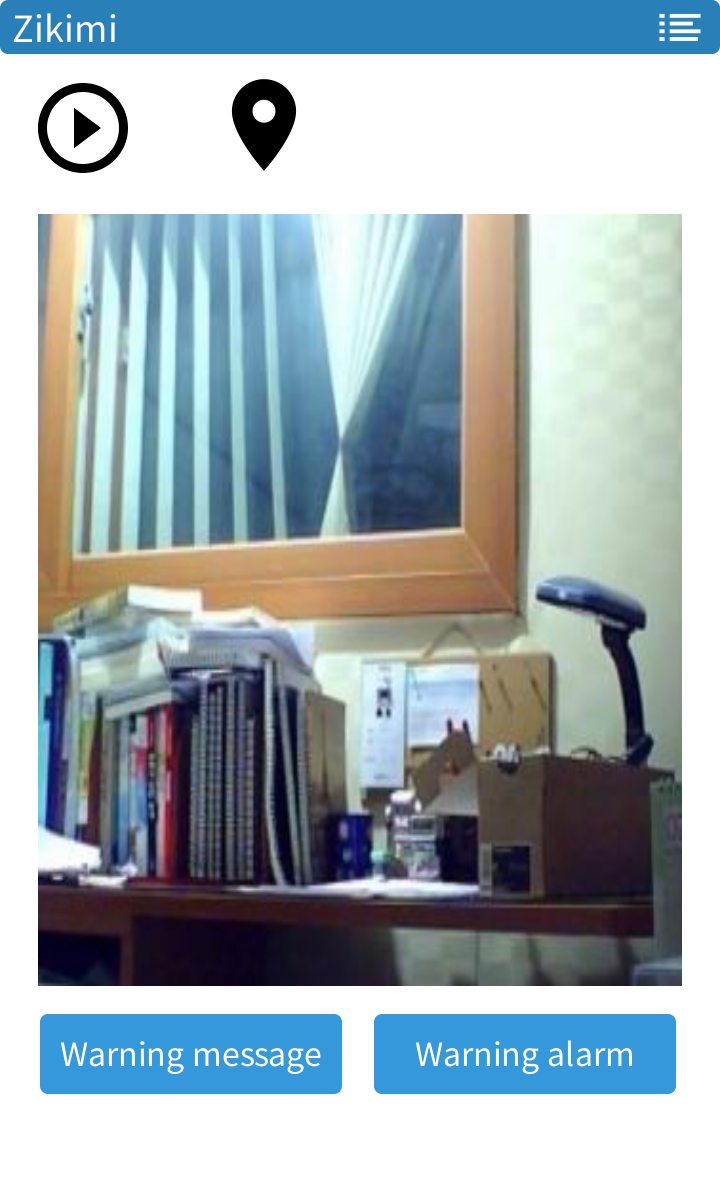
\includegraphics[width=80mm,scale=1.2]{basicstreaming}
\end{center}
\begin{enumerate}
\item Build the streaming server in the laptop. (ex. Install VLC Media Player Streaming Server)\\
\item Building Process\\
 - To find out the android device’s IP address, we should connect it to the laptop USB.\\
 - In the laptop, use CMD.exe ipconfig and find out both laptop’s IP address and android device’s.\\
 - Fix the protocol to RTP / MPEG Transport Stream.\\
 - Video type ->Encapsulate video into MPEG-TS\\
                          Fix the video Codec to MPEG-4\\
                          Fix the audio Codec to MPEG-4 Audio(AAC)\\
 - Enter the IP address of android device where the address of converted stream via RTP should be printed.\\
 - Fix the transcoding profile type to Video – H.264 + AAC(MP4)\\
\item Build the streaming client in the android smartphone. (ex. Stream Media Player)\\
 - Enter the streaming RTSP IP address of your laptop\\
\item Display the video in real time.\\
\end{enumerate}

%Subsubsection 2
\subsubsection{Login / Logout}
\begin{center}
[Log-in page on the android device screen] \\ [1\baselineskip]
\end{center}
\begin{center} 
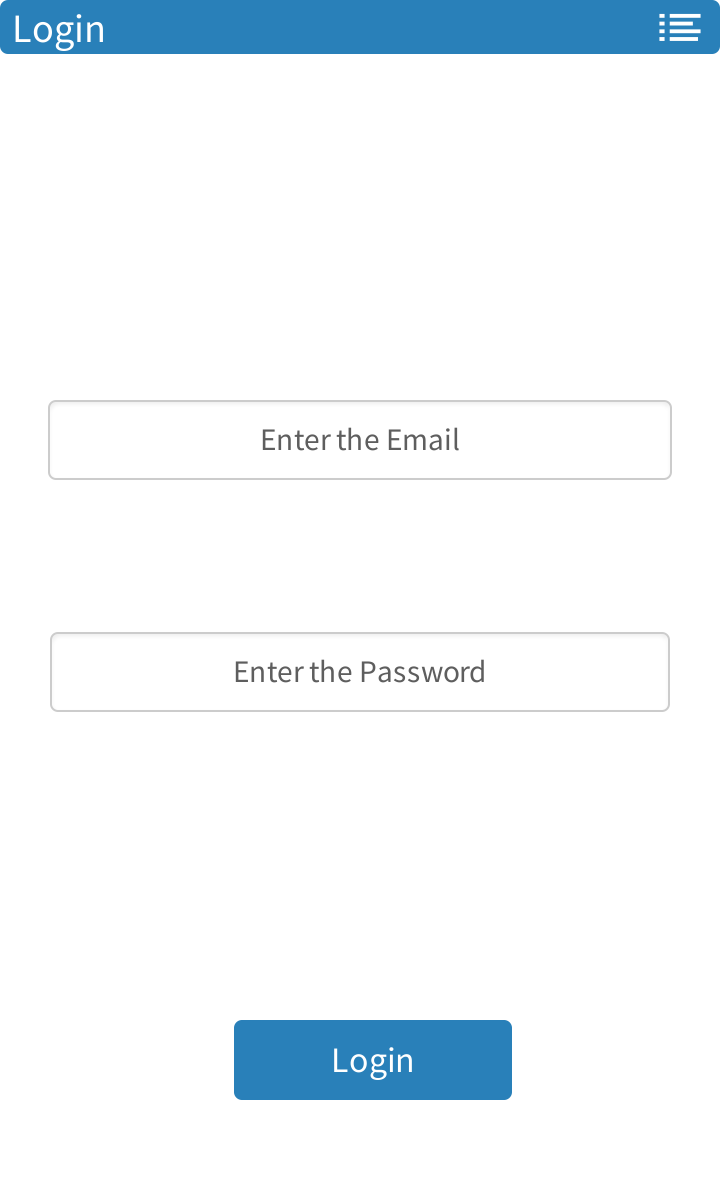
\includegraphics[width=80mm,scale=1.2]{login}
\end{center}
\begin{center}
[ Log-in page on the laptop screen ] \\ [1\baselineskip]
\end{center}
\begin{center} 
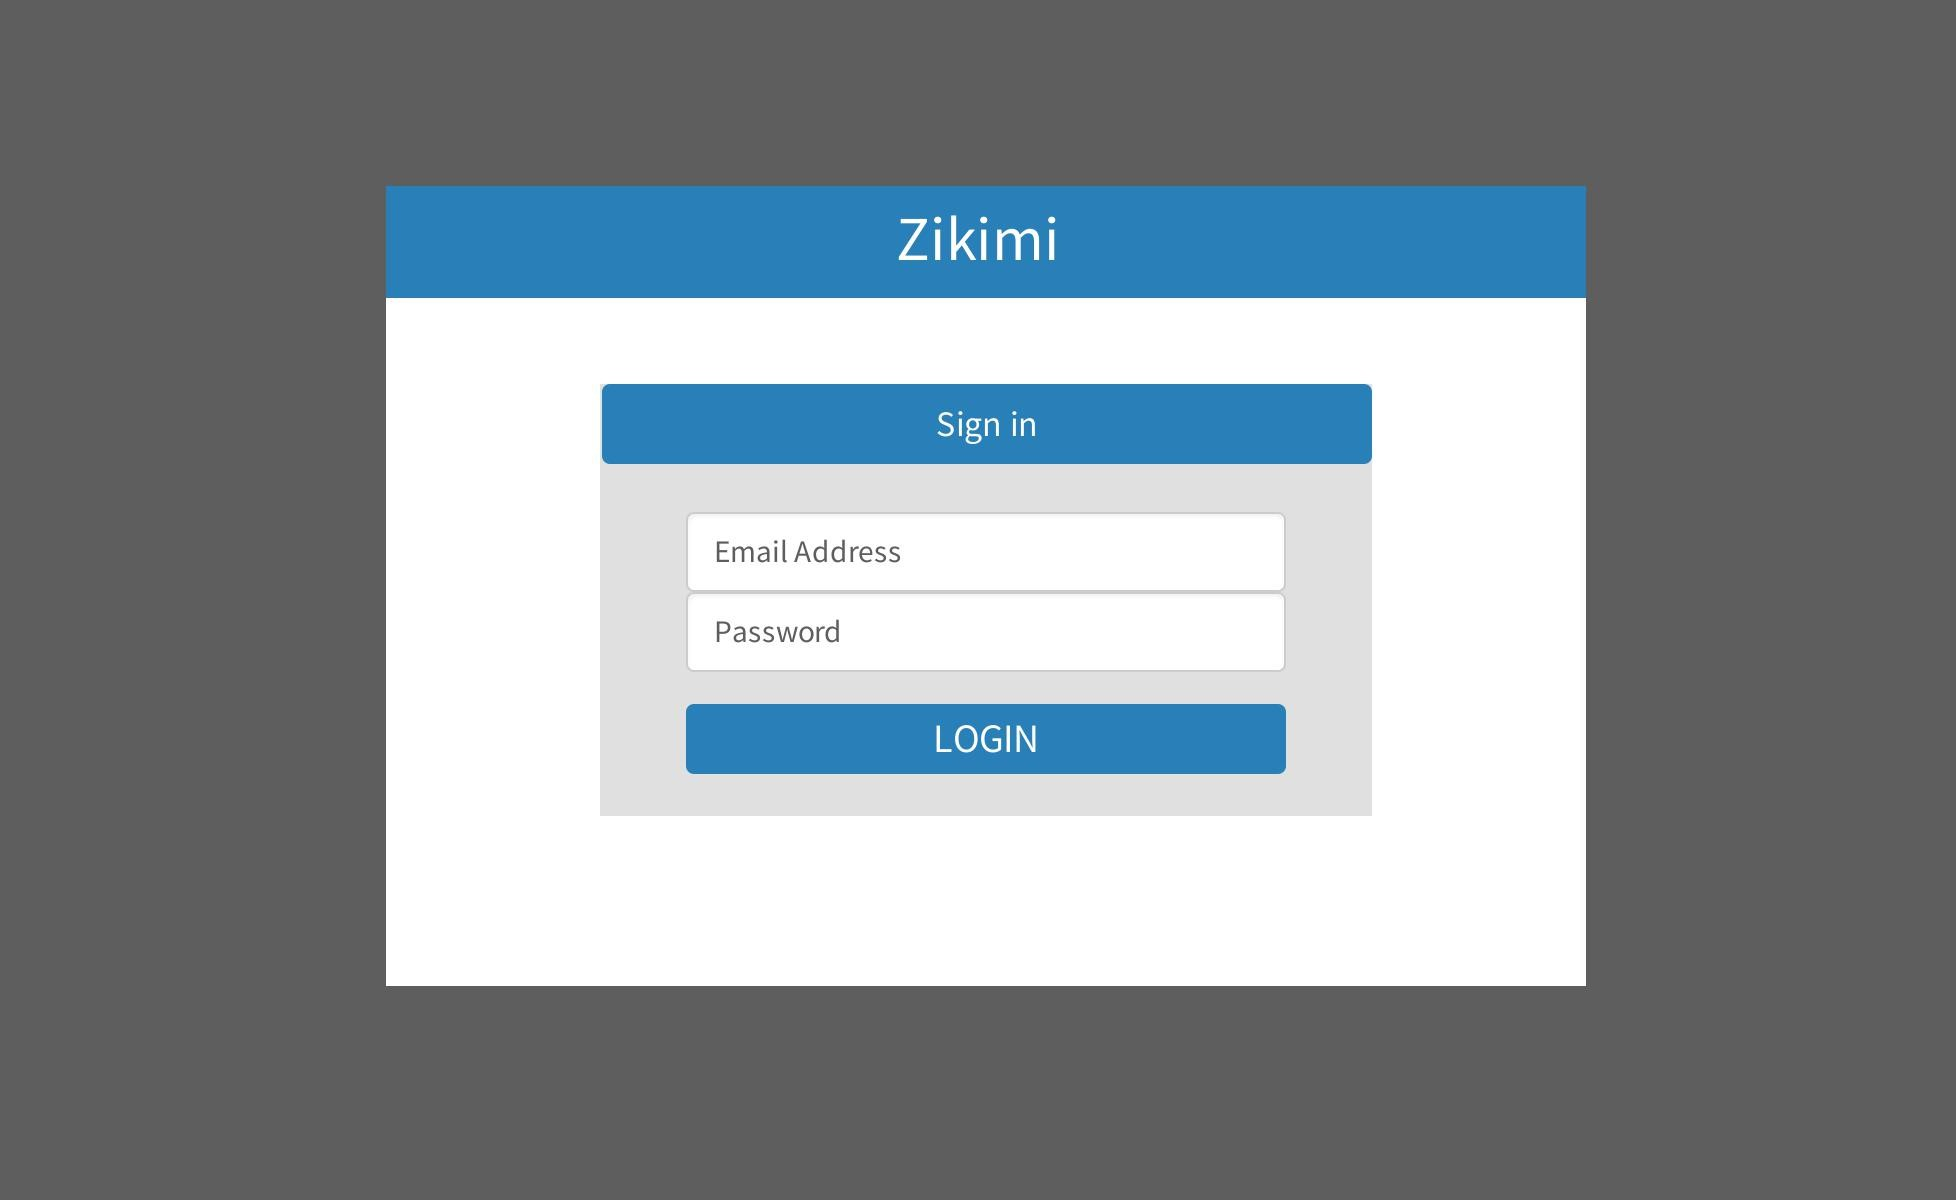
\includegraphics[width=80mm,scale=1.2]{laptoplogin}
\end{center}
\begin{enumerate}
\item Sign up is in the android device
\item Sign up details are e-mail address, password, password confirm, e-mail address duplication confirm.
\item E-mail address type is string, since e-mail addresses’ length are various, fix the e-mail addresses’ length to 255 byte.
\item By using redundancy checking function in PHP, confirm e-mail address redundancy check.
\item Password type is string, more than 6byte, lower than 12byte.
\item Once you log-in, log-in state will be maintained.
\item We can’t sign up in the computer, just log-in is possible.
\item Every time you log-in, android device and computer will be linked, finish to available streaming.
\item And program (Initial Menu Screen) will be executed.
\end{enumerate}

%Subsubsection 3
\subsubsection{Initial Menu Screen}
\begin{center}
[ Initial Menu Screen on the android device ] \\ [1\baselineskip]
\end{center}
\begin{center} 
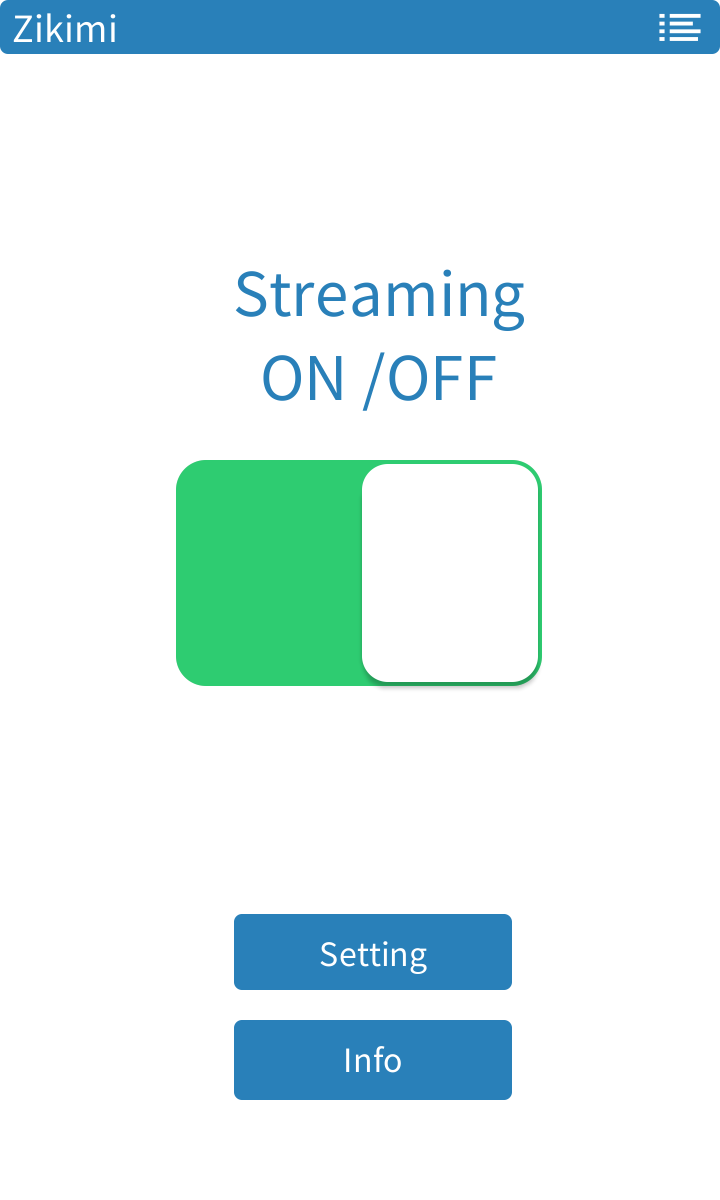
\includegraphics[width=80mm,scale=1.2]{InitialMenuScreen}
\end{center}
\begin{center}
[ Initial Menu Screen on the computer ] \\ [1\baselineskip]
\end{center}
\begin{center} 
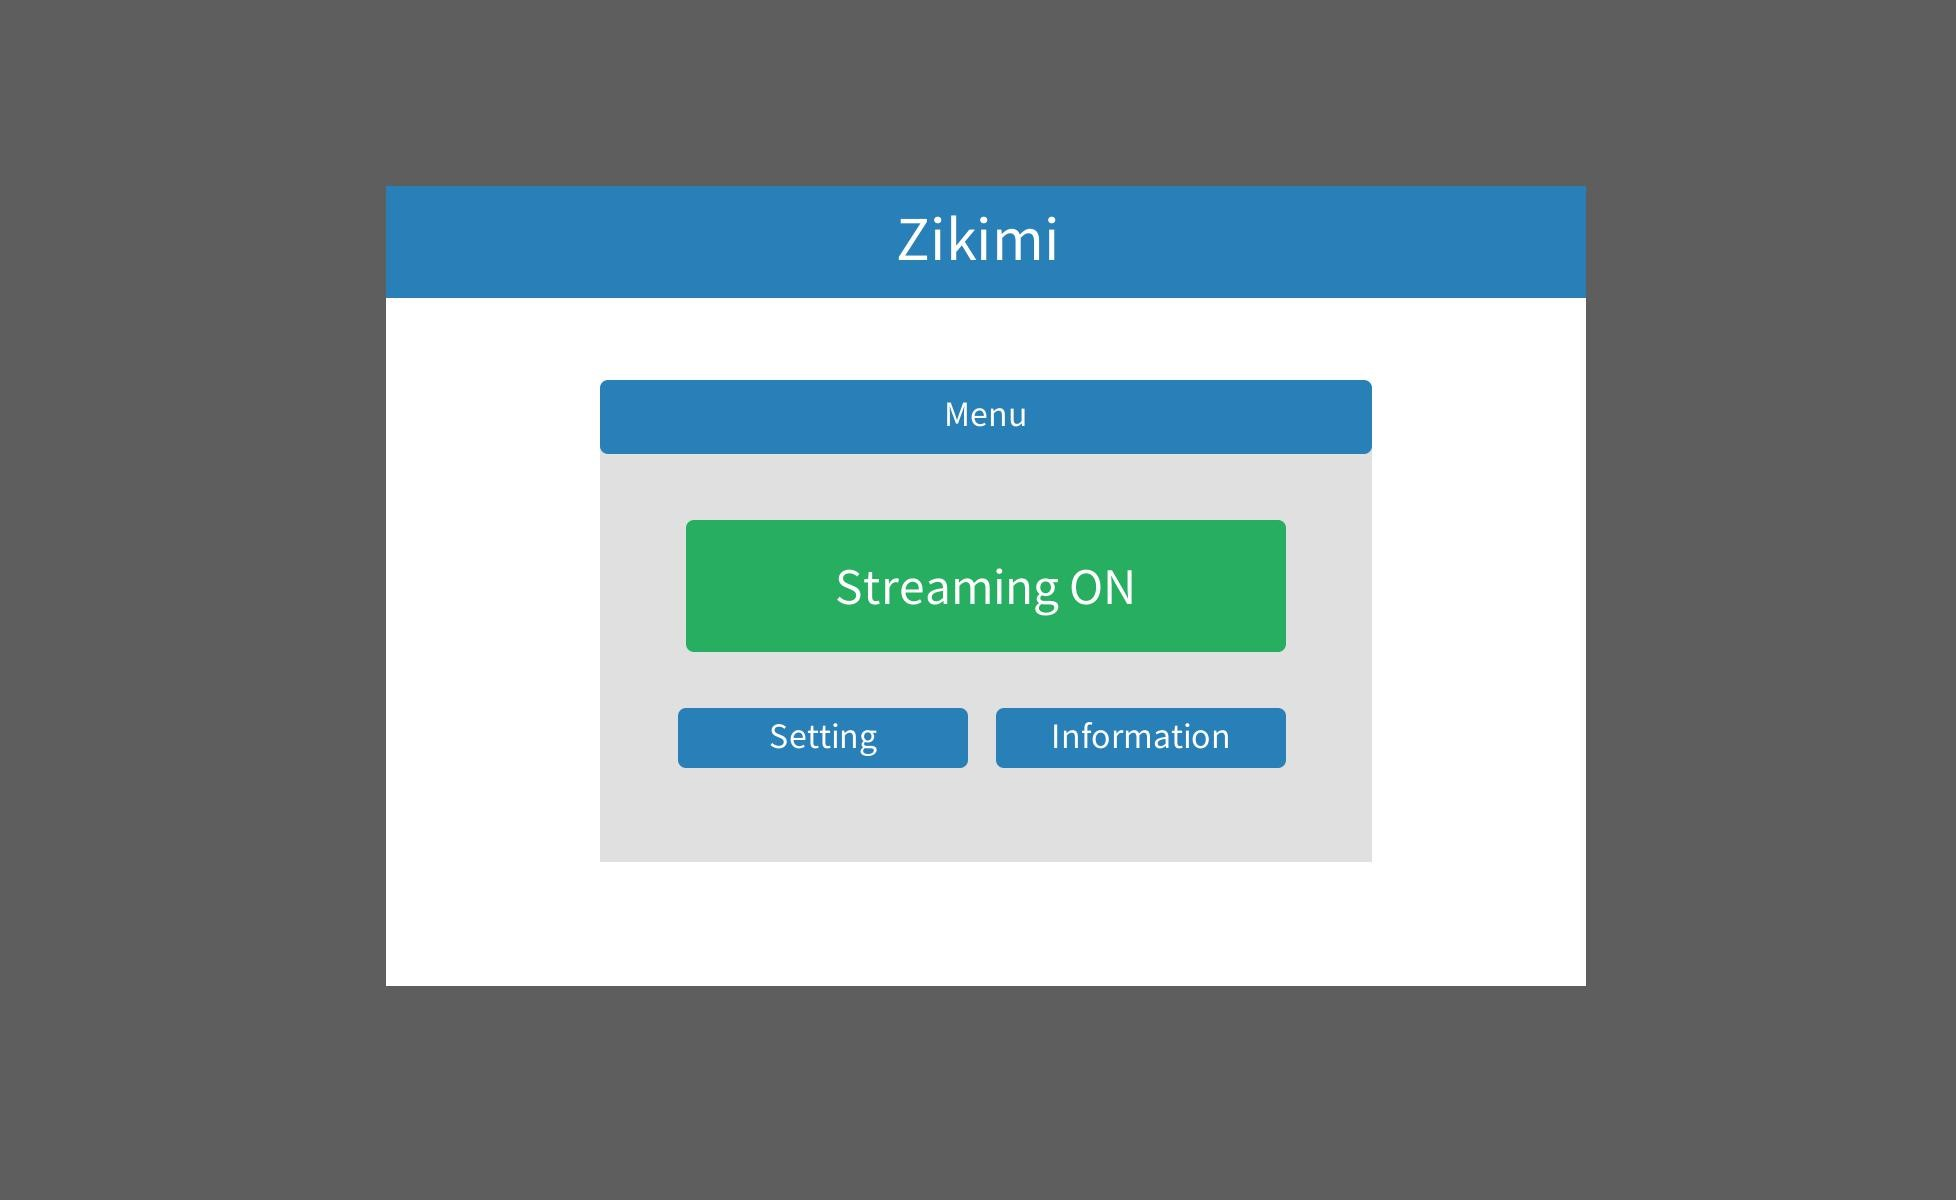
\includegraphics[width=80mm,scale=1.2]{initialmenuscreencomputer}
\end{center}
\begin{enumerate}
\item Screen Size – 600 * 400 pixel (horizontal * vertical)
\item Streaming ON/OFF button
\item Setting – computer tab, android tab
\item Information of developers – our team name and department.
\end{enumerate}

%Subsubsection 4
\subsubsection{Lock Function}
\begin{enumerate}
\item After start streaming in the initial menu screen, all other functions in the laptop will be locked.
\item Background of the screen will be changed into grey screen and we just can move mouse but not clicking.
\end{enumerate}


\subsection{Warning System (from Android to laptop)}
%Subsubsection 1
\subsubsection{Message}
\begin{center} 
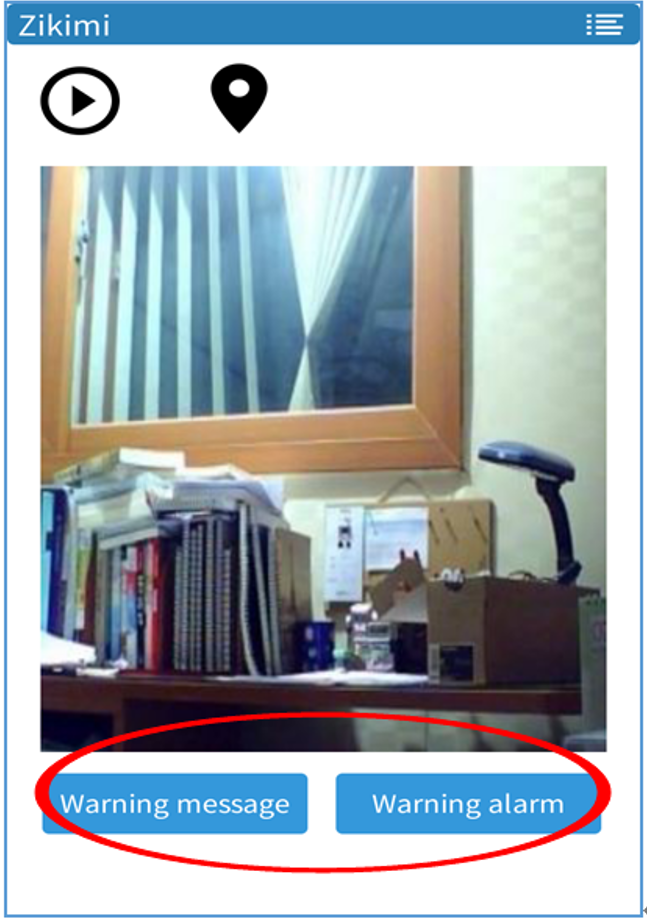
\includegraphics[width=80mm,scale=1.2]{warning}
\end{center}
\begin{enumerate}
\item When someone’s trying to steal the laptop
\item If you click the warning message transmission button in the lower left side of the streaming screen in the android device, the warning message popup will be executed.\\
 - Message window size : 1200 * 800 pixels\\
 - Contents of warning message : At the middle of the top section, ‘Warning’, below that, ‘Now, I see you. Don’t touch!\\
\begin{center} 
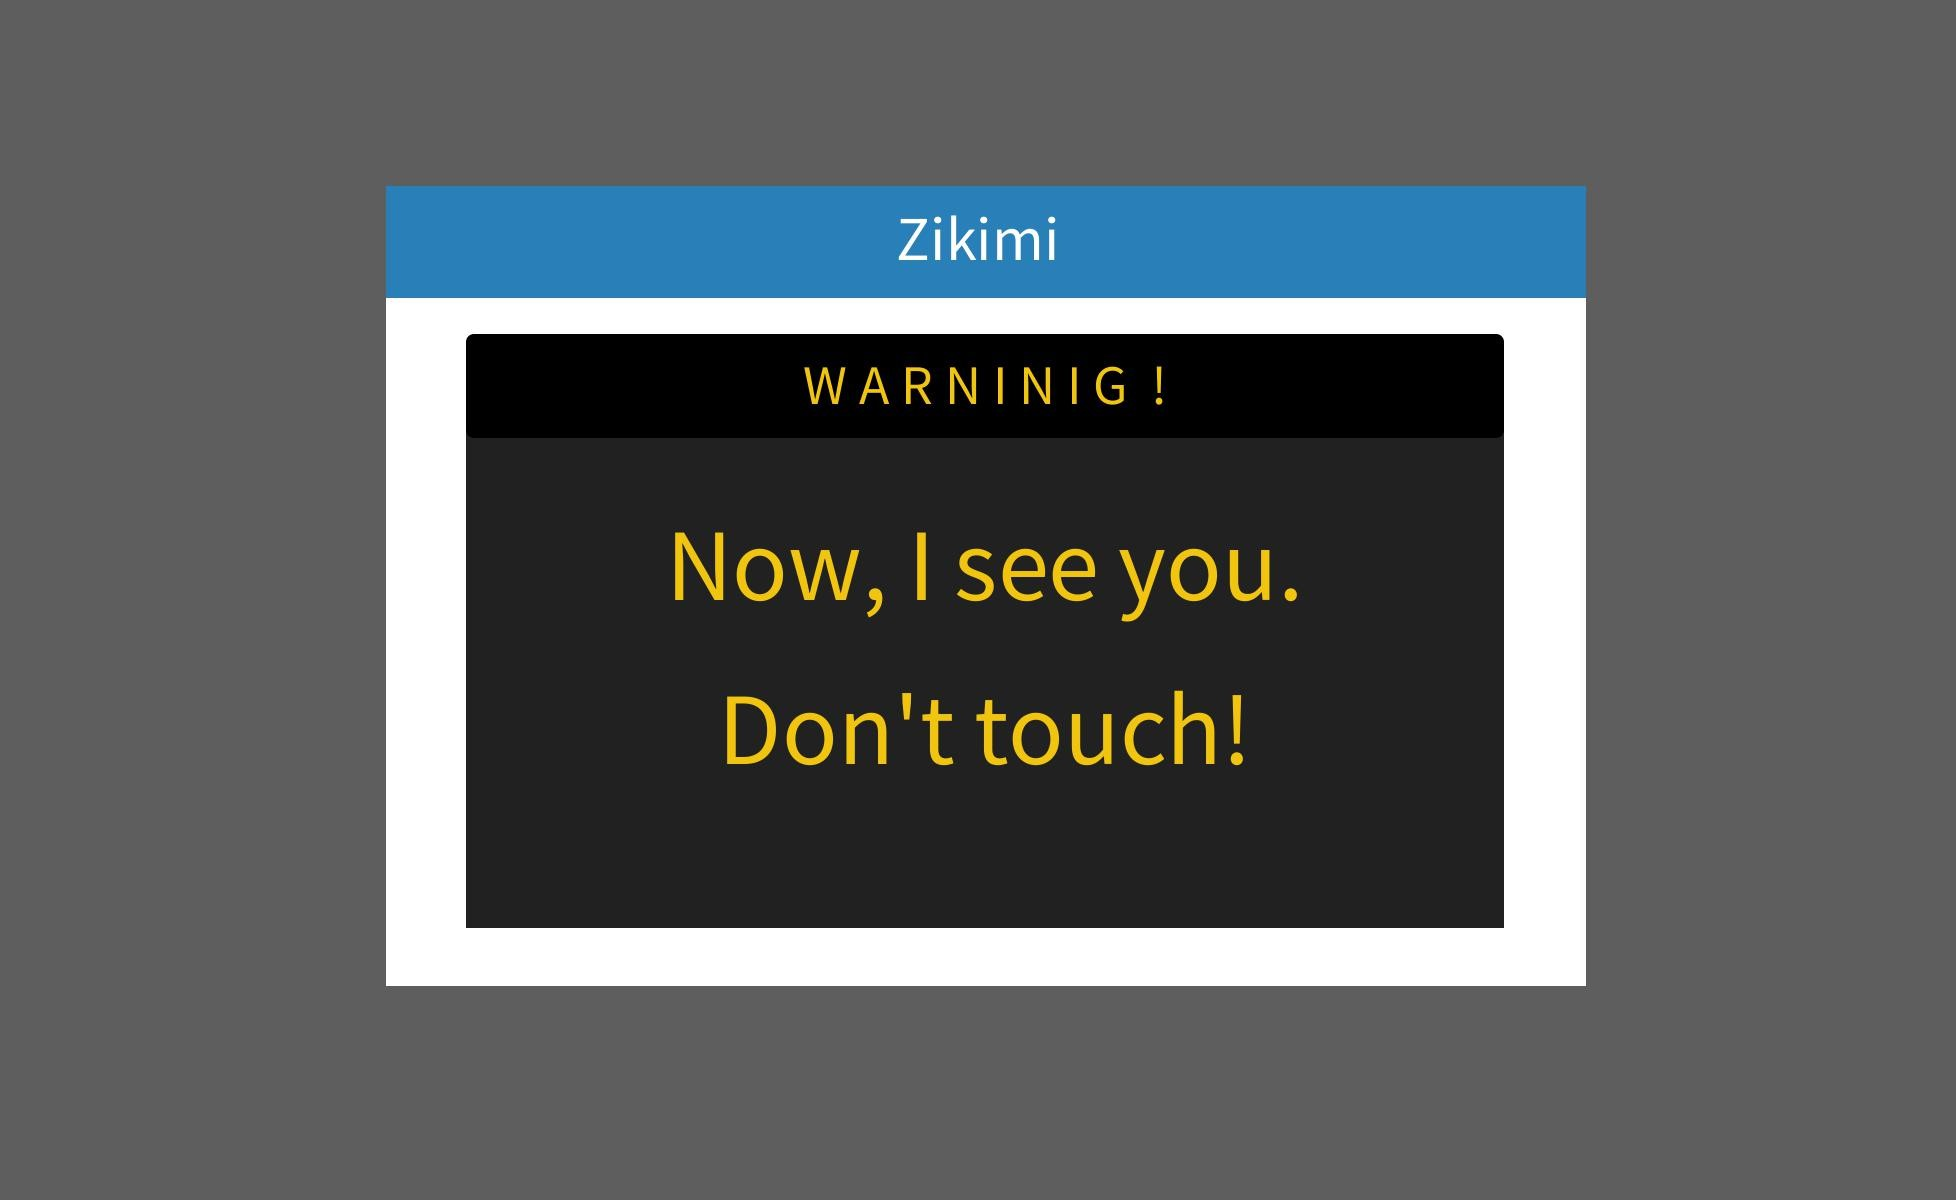
\includegraphics[width=80mm,scale=1.2]{warningmessage}
\end{center}
\item If you click the warning message transmission button again, the popup will be shut down.
\end{enumerate}

%Subsubsection 2
\subsubsection{Warning Alarm}
\begin{enumerate}
\item When someone’s trying to steal the laptop
\item Click the warning alarm button at the bottom and right side of the streaming screen in your android device.
 - Warning alarm : 70 decibel, continue until the turning off, beep…beep…sound.
\item Click the warning alarm button again, it will be shut down.
\end{enumerate}

\subsection{Situation Reporting System}
%Subsubsection 1
\subsubsection{Battery under 10percent}
\begin{center} 
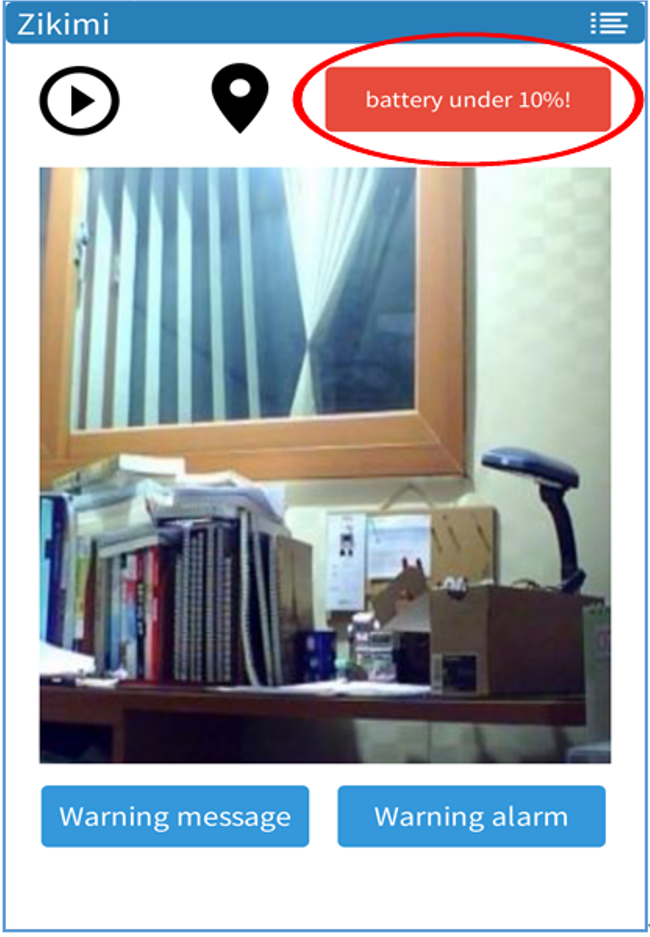
\includegraphics[width=80mm,scale=1.2]{battery}
\end{center}
\begin{enumerate}
\item When the battery of the laptop is lower than 10percent\\
\item Send the popup message to the android device\\
\item This message will be shown at the top and the right side of the streaming screen\\
 - Message window size : 150 * 100 pixels\\
 - Contents of the message : ‘Battery under 10percent!’\\
\end{enumerate}

%Subsubsection 2
\subsubsection{Charger removed}
\begin{center} 
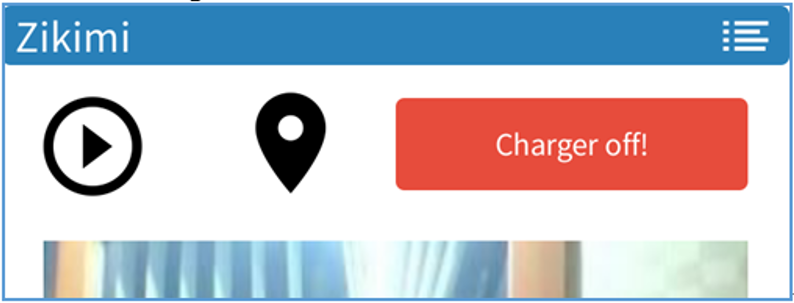
\includegraphics[width=80mm,scale=1.2]{charger}
\end{center}
\begin{enumerate}
\item When someone removed the laptop charger
\item Send the popup message to the android device
\item This message will be shown at the top and the right side of the streaming screen\\
 - Message window size : 150 * 100 pixels\\
 - Contents of the message : ‘Charger removed!’\\
 - Warning message window size in the computer : 1200 * 800 pixels\\
- Contents of warning message : At the middle of the top section, ‘Warning’, below that, ‘Now, I see you. Don’t touch!’\\
\end{enumerate}

%Subsubsection 3
\subsubsection{USB removed}
\begin{center} 
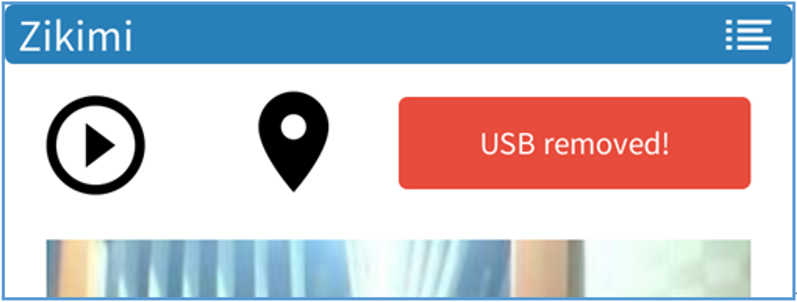
\includegraphics[width=80mm,scale=1.2]{usbremoved}
\end{center}
\begin{enumerate}
\item When someone removed USB
\item Send the popup message to the android device
\item This message will be shown at the top and the right side of the streaming screen\\
 - Message window size : 150 * 100 pixels\\
 - Contents of the message : ‘USB removed!’\\
- Warning message window size in the computer : 1200 * 800 pixels\\
- Contents of warning message : At the middle of the top section, ‘Warning’, below that, ‘Now, I see you. Don’t touch!’\\
\end{enumerate}

%Subsubsection 4
\subsubsection{Mouse moved}
\begin{center} 
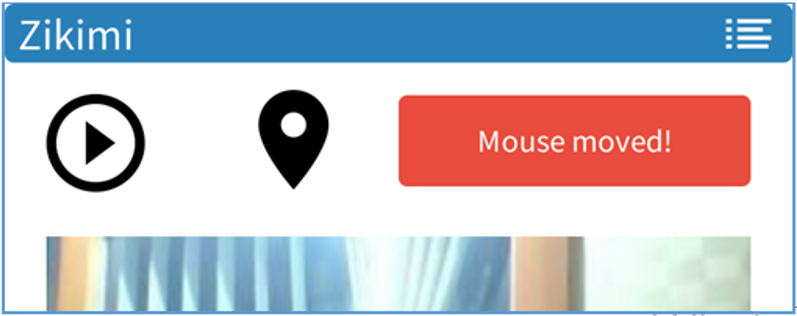
\includegraphics[width=80mm,scale=1.2]{mousemoved}
\end{center}
\begin{enumerate}
\item When someone moved mouse more than 10 pixels from x-axis and y-axis\\
\item Send the popup message to the android device\\
\item This message will be shown at the top and the right side of the streaming screen\\
 - Message window size : 150 * 100 pixels\\
 - Contents of the message : ‘Mouse moved!’\\
 - Warning message window size in the computer : 1200 * 800 pixels\\
- Contents of warning message : At the middle of the top section, ‘Warning’, below that, ‘Now, I see you. Don’t touch!’\\
\end{enumerate}

%Subsubsection 5
\subsubsection{Keyboard typed}
\begin{center} 
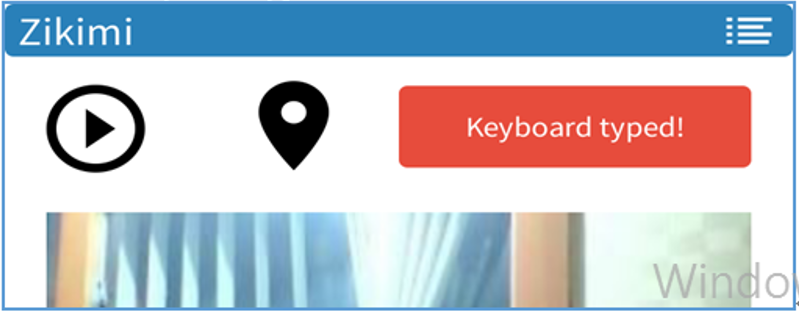
\includegraphics[width=80mm,scale=1.2]{keyboard}
\end{center}
\begin{enumerate}
\item When someone beat the button more than one\\
\item Send the popup message to the android device\\
\item This message will be shown at the top and the right side of the streaming screen\\
 - Message window size : 150 * 100 pixels\\
 - Contents of the message : ‘Keyboard typed!’\\
 - Warning message window size in the computer : 1200 * 800 pixels\\
- Contents of warning message : At the middle of the top section, ‘Warning’, below that, ‘Now, I see you. Don’t touch!’\\
\end{enumerate}

%Subsubsection 6
\subsubsection{Socket Programming in JAVA}
We will use JAVA’s socket programming in Warning System and Situation Reporting System when the laptop and the android device send messages each other.\\
JAVA provides various types of classes for people to implement socket programming easily. We can get IP address, domain, host name by using InetAddress class. With getHostAddress () method of this class we can get the address of the host to STRING. We are going to use it. And then we will implement a socket server using the ServerSocket class. And the socket on the client side will be implemented using the Socket class.\\

\subsection{Recording Function (Control recording through Android)}
\begin{center} 
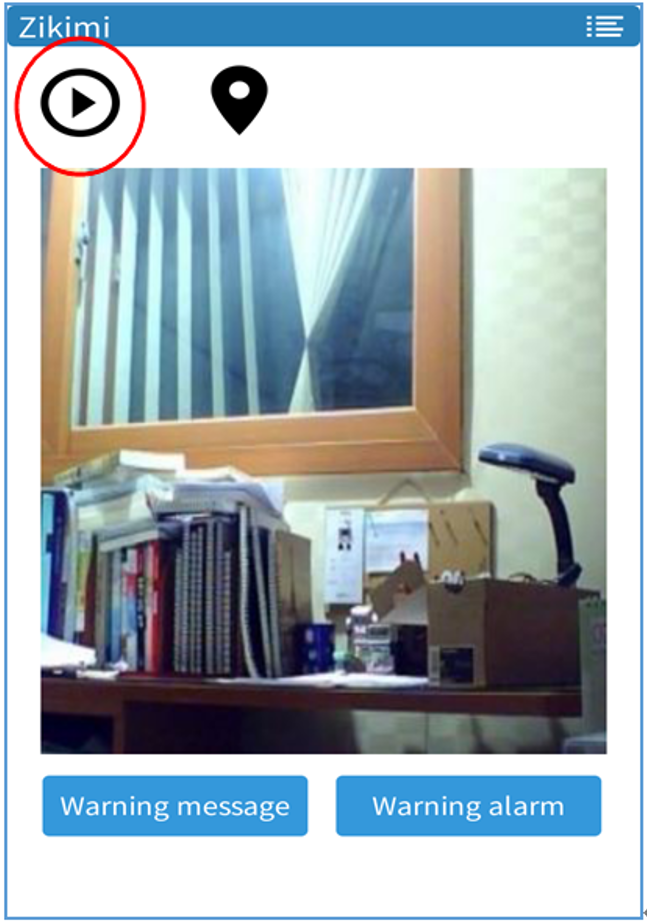
\includegraphics[width=80mm,scale=1.2]{record}
\end{center}
\begin{enumerate}
\item In the event of theft or situations that require recording\\
\item Control recording on android device via the Record button (REC. ON / OFF) in order to leave the proof of theft.\\
\item This button is located on the top left\\
\item The recorded video is automatically saved to the sd card first on Android devices.\\
\item When the sd card is not attached\\
 - Automatically saved internal storage on the android device\\
\item Image length ( size ) is limited to 30 minutes.\\
 - The capacity of resolution in streaming parts will be decided later.\\
\end{enumerate}

\subsection{Location Tracking (The last resort)}
\begin{center} 
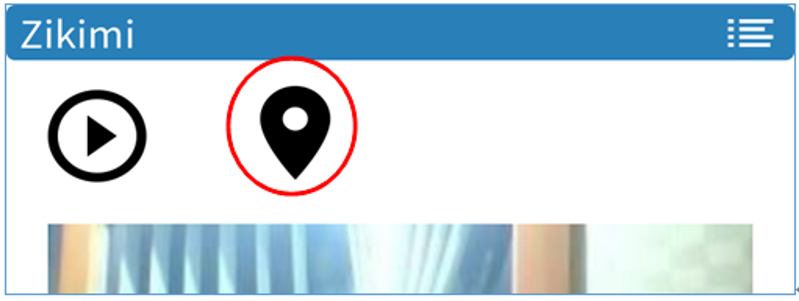
\includegraphics[width=80mm,scale=1.2]{location}
\end{center}
\begin{enumerate}
\item If none of the earlier anti-theft alarm and warning messages are effective, you can track the location of your laptop as a last resort.
\item Tracking Start button is located on top center of the Android screen.
\item After you press the Start button, the location of laptop will be sent per 1 minute to the android device as a message.
\end{enumerate}



%Section
\newpage\section{Architecture Design and Implementation(Partial)}

\subsection*{Overall Architecture}
\begin{center} 
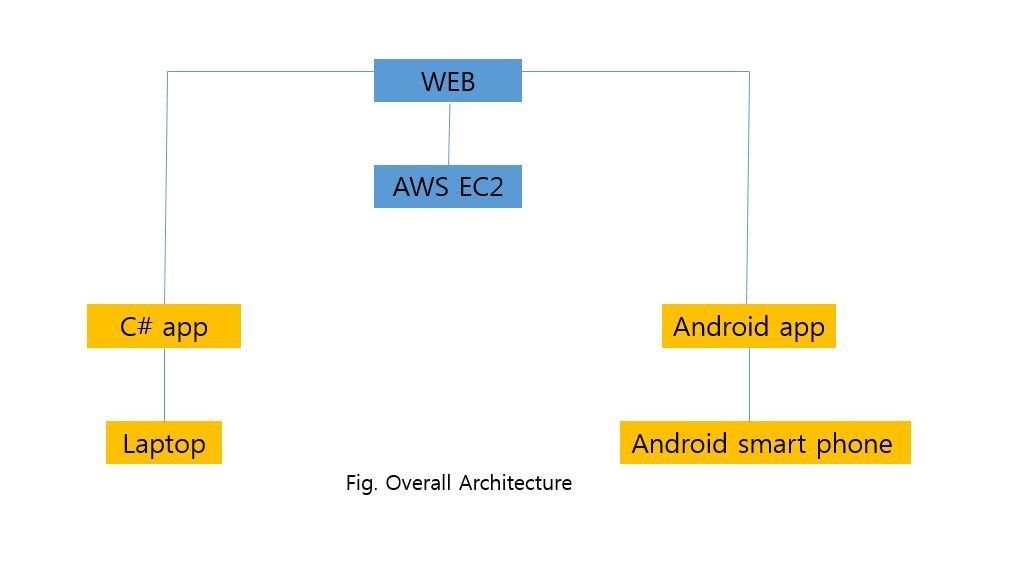
\includegraphics[width=140mm,scale=1.8]{overallarchitecture}
\end{center}
Using the Amazon EC2 web server communicate between C-Sharp and Android. Use the Web RTC technology to stream two images.
\subsection*{Web Architecture}
\begin{center} 
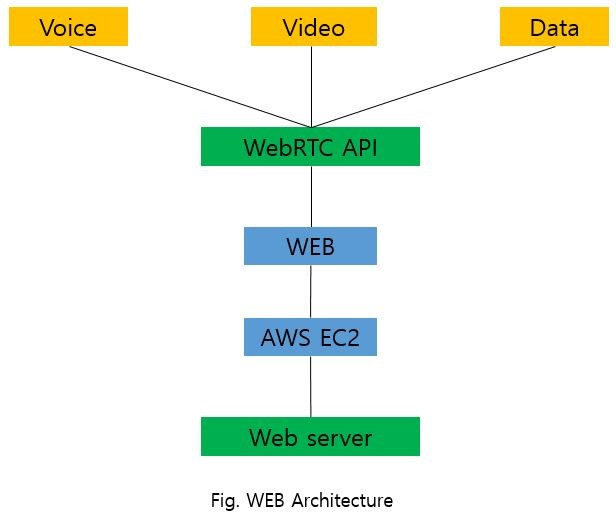
\includegraphics[width=120mm,scale=1.8]{webarchitecture}
\end{center}
\begin{enumerate}
\item Amazon Web Service EC2 - Web server\\
\\
It uses the EC2 Cloud computing service provided by Amazon Web Service to the Web server. Using the EC2 computer to build a Web server environment.\\
\item Web RTC API\\
\\
Web RTC (Web Real - Time Communication) is an API that is designed to communicate with each other without the help of a web browser plug-in between. The draft presented at the W3C, which can be used as voice calls, video calls, P2P file sharing. The Media streaming (Voice, Video), Data transfer function between the user which is provided by Web RTC will implement real-time video communication and message transmission between Laptop and Android Smart-phone. Through the Web server built into EC2, we will use Web RTC API.
\\
\end{enumerate}

\subsection*{Laptop Architecture}
\begin{center} 
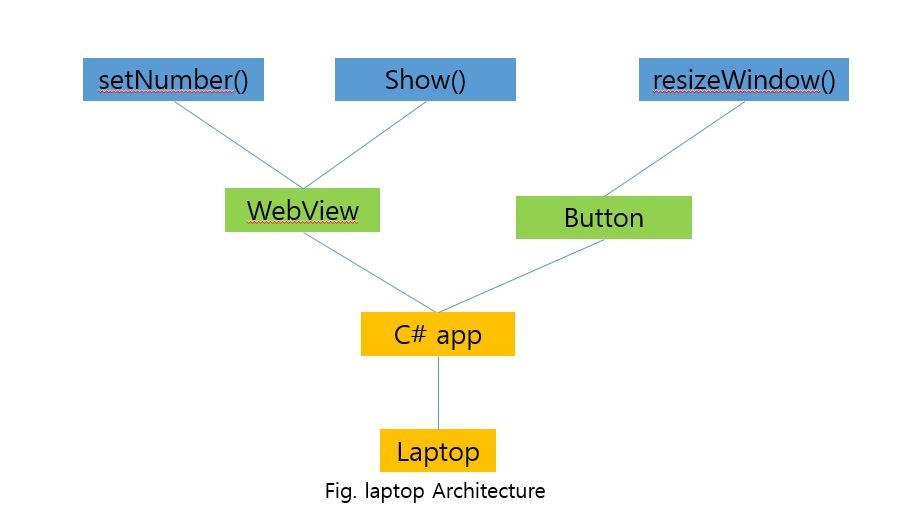
\includegraphics[width=120mm,scale=1.8]{laptoparchitecture}
\end{center}
\begin{enumerate}
\item WebView\\
\\
 WebView contain streaming web that used webrtc api. And it has two methods. First thing is setNumber(). This method get special number from user. This number will be used at android to see the laptop’s camera screen. Second thing is Show(). This method is used at show the contents of streaming screen.\\

\item Button\\
\\
Button is used to resize the C-Sharp program screen at minimum. To hide the laptop’s camera screen at laptop. User must use this button to hide their camera screen. \\
\end{enumerate}

\subsection*{Android Architecture}
\begin{center} 
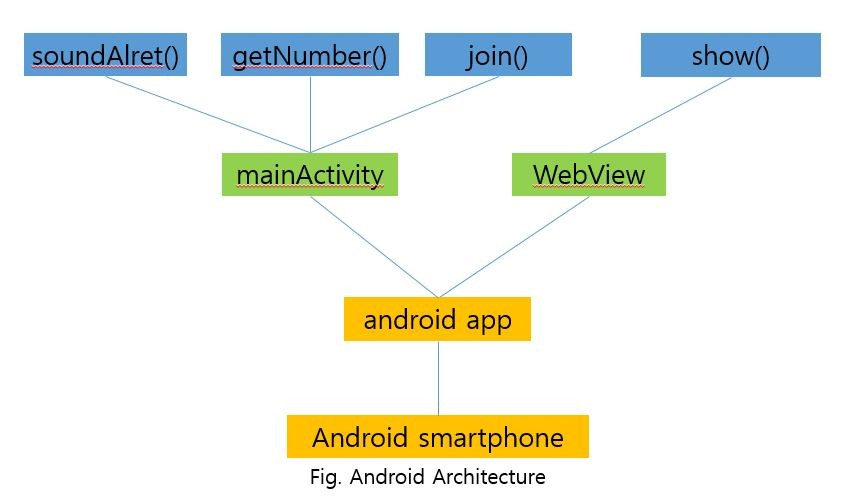
\includegraphics[width=120mm,scale=1.8]{androidarchitecture}
\end{center}
\begin{enumerate}
\item mainActivity\\
\\
It has three methods. First thing is soundAlert. User can see the thieves by android application. So if user see the thieves, user can push the soundAlert button to ring the alert bell at the laptop. Second thing is getNumber. User can get number from laptop by this method. Third thing is join. User can connect to the laptop by this method.\\

\item Web View\\
\\
WebView contain one method that is Show(). This method is used at show the contents of streaming screen from laptop.\\
\end{enumerate}

\subsection*{Directory Organization}
\begin{center} 
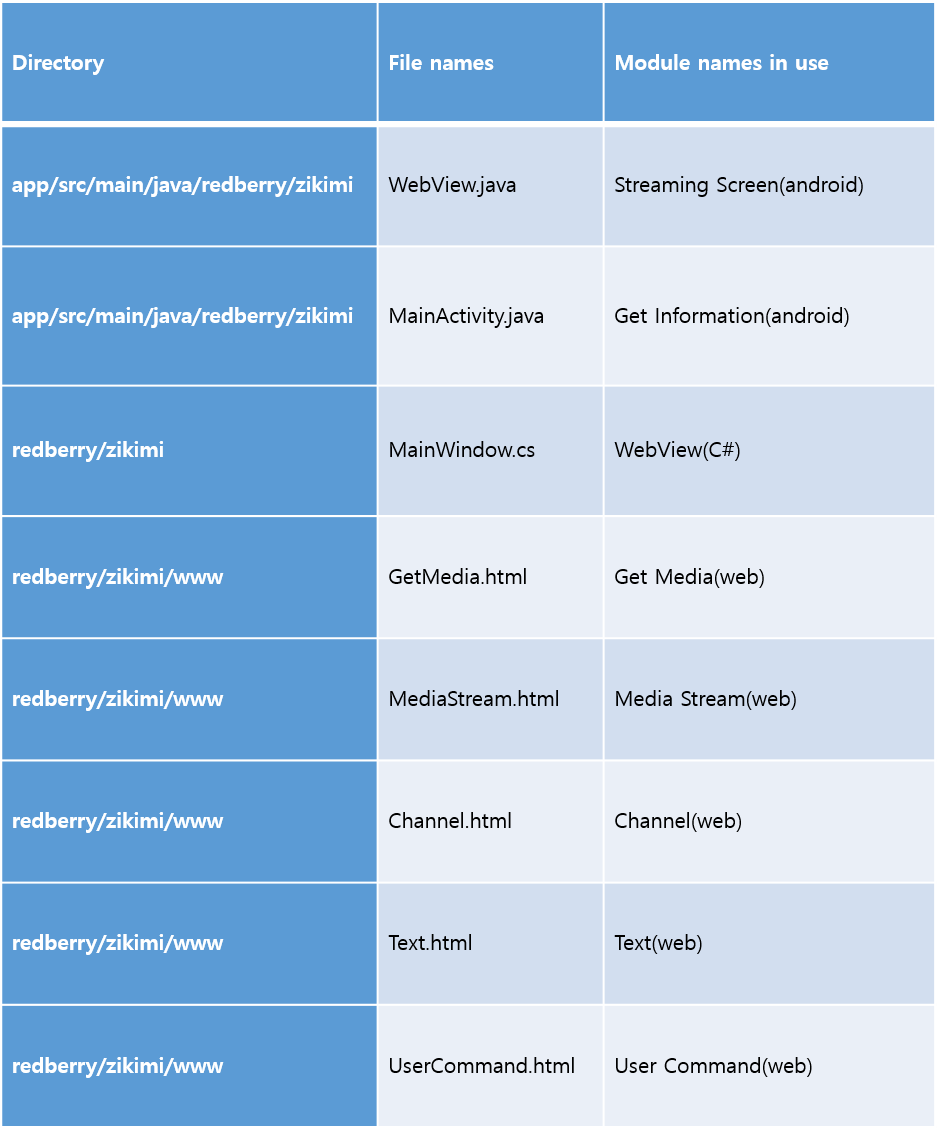
\includegraphics[width=120mm,scale=1.8]{directory}
\end{center}



\subsection*{Module}
\begin{enumerate}
\item Streaming Screen(Android)\\
\\
In this module user can see the streaming screen from the laptop camera. \\

\item Main Activity(Android)\\
\\
In this module, user can input the number that set at the laptop computer. If number is correct, user can get streaming screen from the laptop camera. And user can ring the bell to the laptop computer by press the button.\\

\item Web View(C-Sharp)\\
\\
In this module, C-Sharp load the Web View. In the Web View, user can set the number and enter the streaming room.\\

 \item Get Media(Web)\\
\\
This module which is provided by WEB RTC brings the laptop's videos and voices. This module is for taking the videos and voices which is recorded in the laptop webcam to the Web.\\

\item Media Stream(Web)\\
\\
This module which is provided by WEB RTC enables video communication and voice communication between the peers using Video tag.(P2P).\\

\item Channel(Web)\\
\\
This module which is provided by WEB RTC makes the essential channel for communication, brings the channel list and shows.\\

\item Text(Web)\\
\\
This module which is provided by WEB RTC enables giving and receiving Text between the users through the data channel.\\

\item User Command(Web)\\
\\
This module which is provided by WEB RTC delivers commands to the opposite side through the Web Socket based API.\\

\end{enumerate}






%Use Case

\newpage\section{Use Case}
\subsection{Streaming}
\begin{center} 
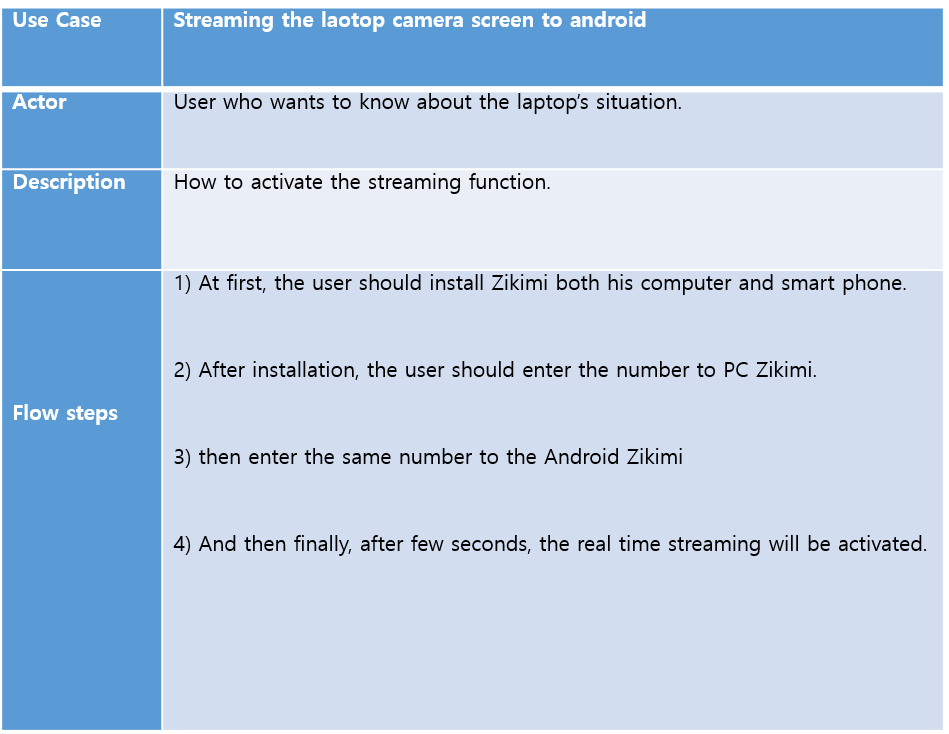
\includegraphics[width=120mm,scale=1.8]{streaming}
\end{center}
\begin{itemize}

\item\textbf{Step2}\\ 
\begin{center}
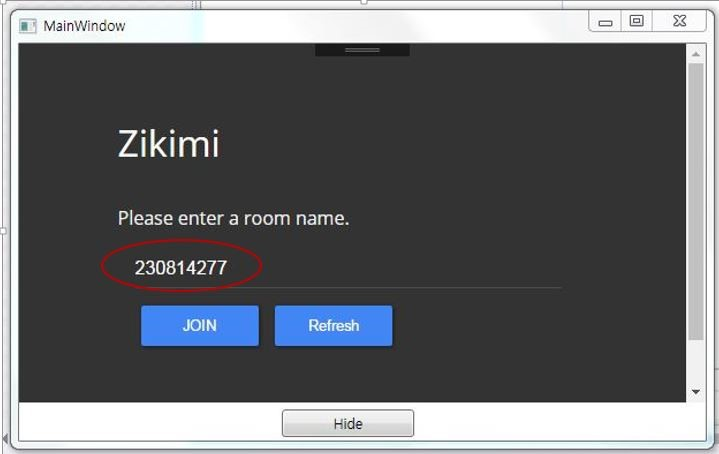
\includegraphics[width=120mm,scale=1.8]{streamingstep2}
\end{center}
\newpage
\item\textbf{Step3}\\
 \\ 

\begin{center} 
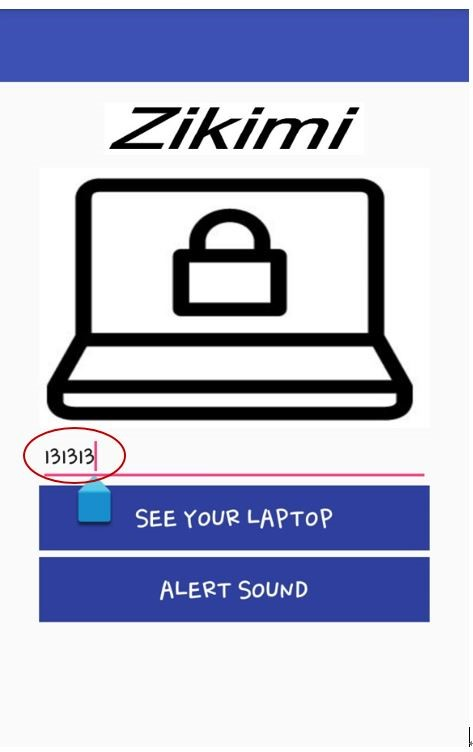
\includegraphics[width=60mm,scale=1]{streamingstep3}
\end{center}

\item\textbf{Step4}\\
\begin{center} 
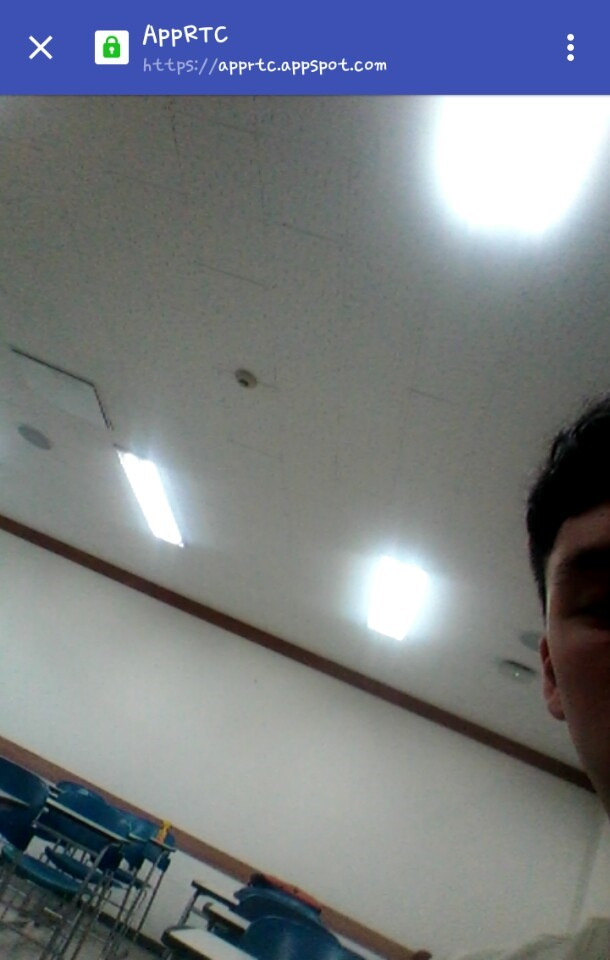
\includegraphics[width=60mm,scale=1]{streamingstep4}
\end{center}
\end{itemize}
\newpage
\subsection{Warning System}
\begin{center} 
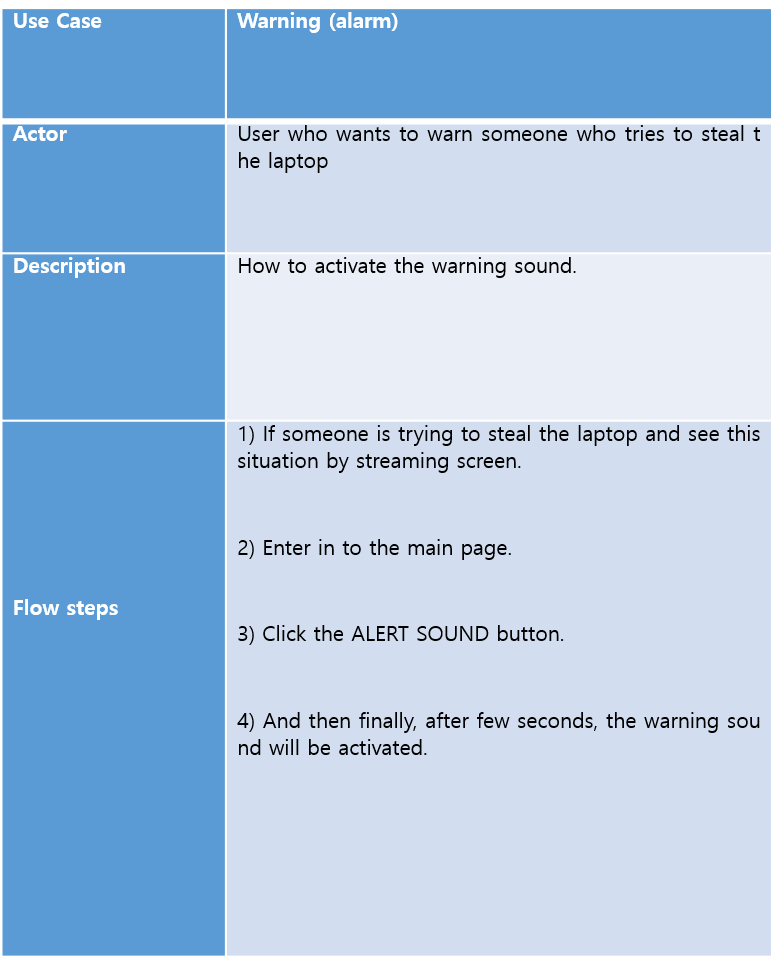
\includegraphics[width=120mm,scale=1.8]{warningsystem}
\end{center}
\newpage
\begin{itemize}

\item\textbf{Step1}\\ 
\begin{center}
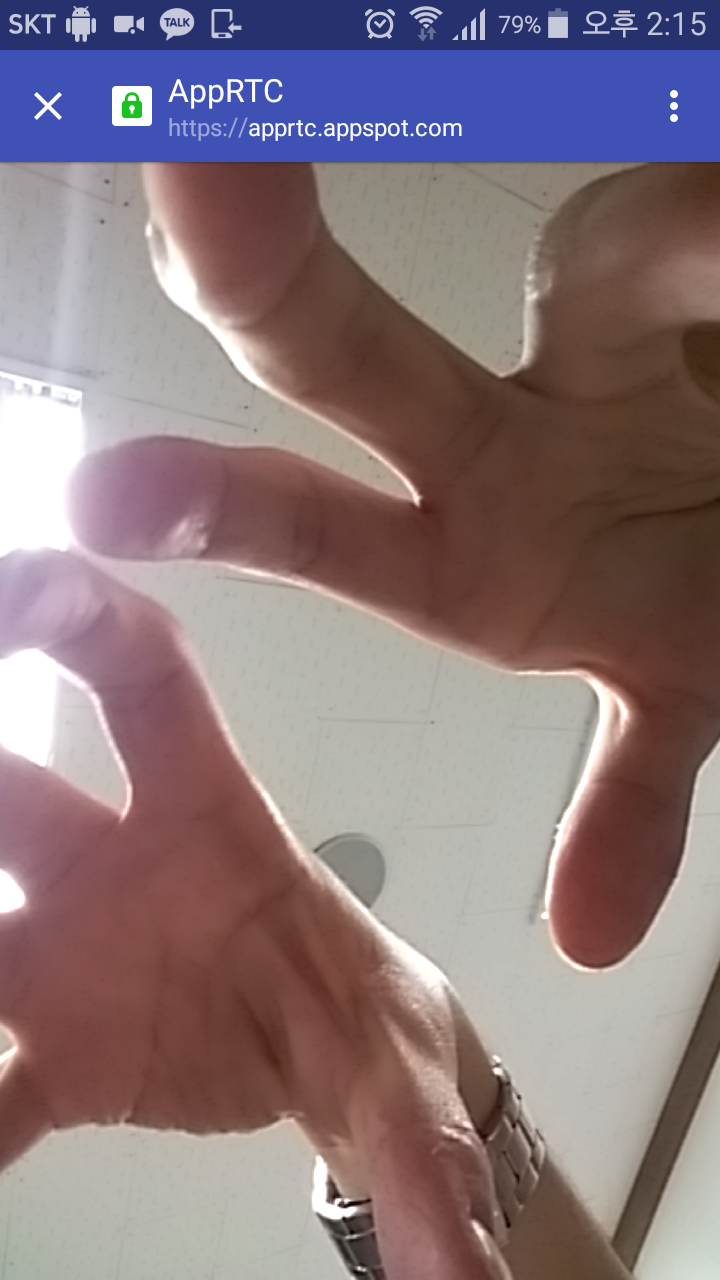
\includegraphics[width=60mm,scale=1]{warningstep1}
\end{center}
\item\textbf{Step3}\\
 \\ 

\begin{center} 
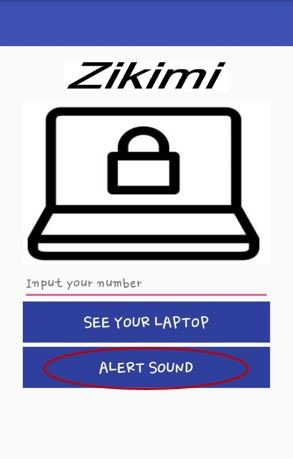
\includegraphics[width=60mm,scale=1]{warningstep3}
\end{center}

\end{itemize}





%Installation Guide
\newpage\section{Installation Guide}
\subsection{Install Visual Studio}
\begin{center}
Go to  http://www.microsoft.com and download the file\\ [1\baselineskip]
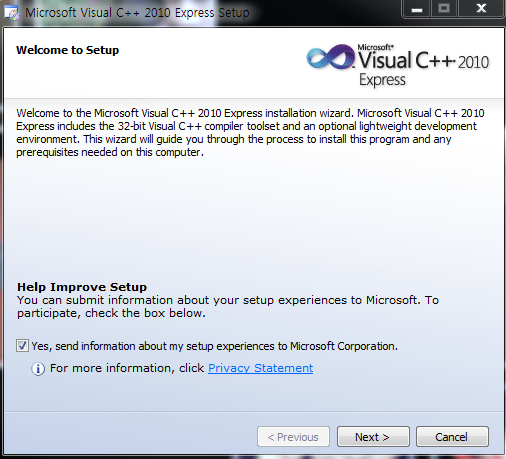
\includegraphics[width=80mm,scale=1.3]{visual1}
\end{center}

\begin{center}
read and accept the license terms, press next. \\ [1\baselineskip]
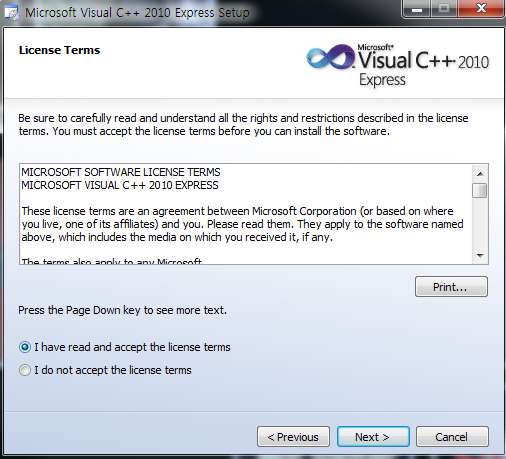
\includegraphics[width=80mm,scale=1.3]{visual2}
\end{center}
\newpage
\begin{center}
Don't check sql server installation, press next\\ [1\baselineskip]
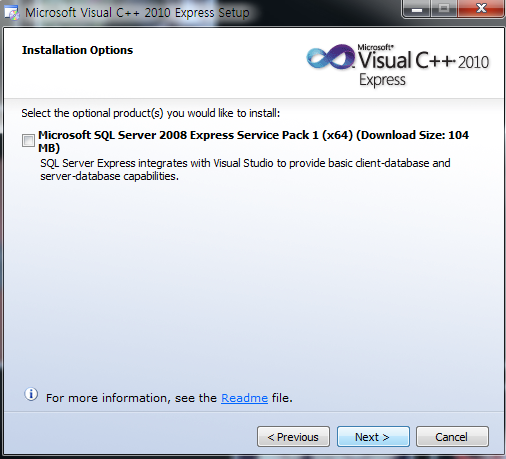
\includegraphics[width=80mm,scale=1.3]{visual3}
\end{center}

\begin{center}
Press install\\ [1\baselineskip]
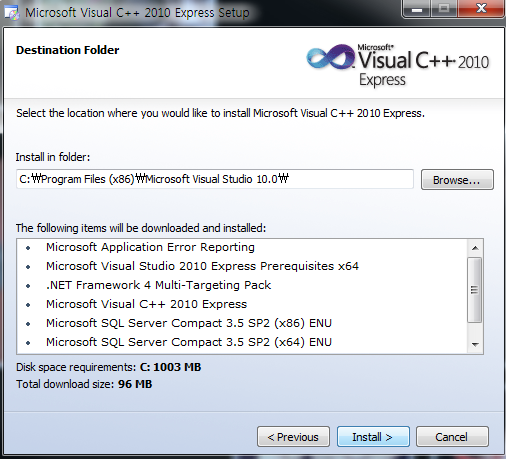
\includegraphics[width=80mm,scale=1.3]{visual4}
\end{center}
\newpage
\begin{center}
Setup complete\\ [1\baselineskip]
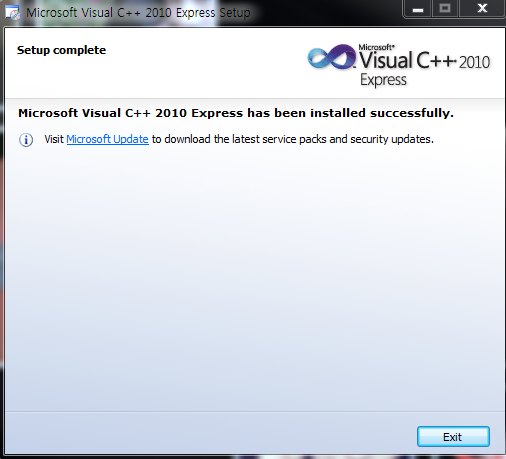
\includegraphics[width=80mm,scale=1.3]{visual5}
\end{center}
\begin{center}
Initial start screen\\ [1\baselineskip]
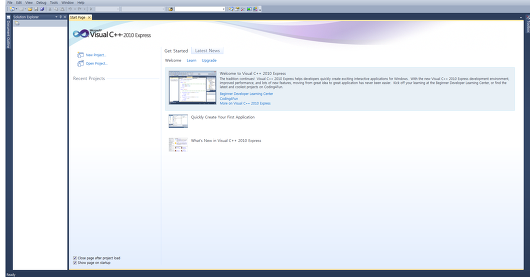
\includegraphics[width=80mm,scale=1.3]{visual6}
\end{center}

\subsection{Install Android Studio}
\begin{center}
Go to Android site and download the file\\ [1\baselineskip]
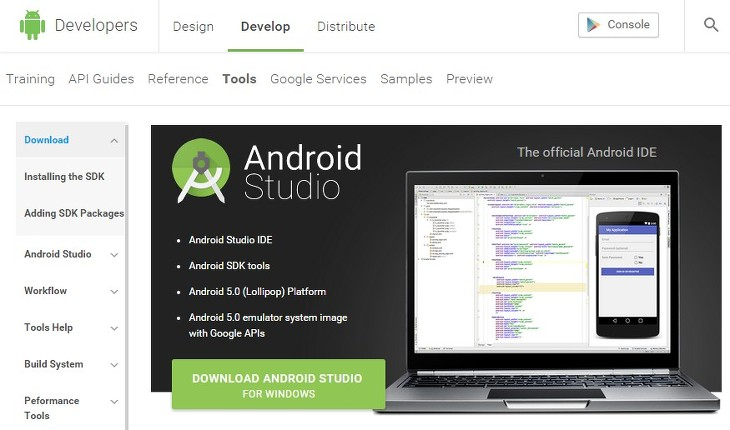
\includegraphics[width=80mm,scale=1.3]{android1}
\end{center}
\newpage

\begin{center}
From now on, in every steps, remain basic setting and just follow until finish\\ [1\baselineskip]
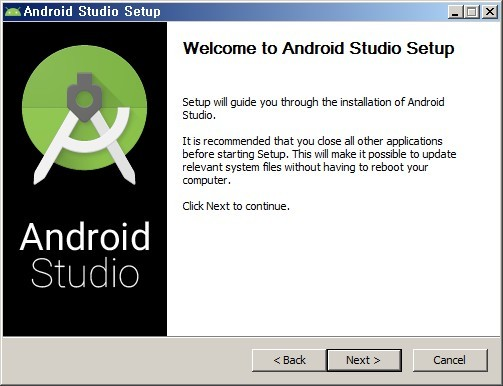
\includegraphics[width=80mm,scale=1.3]{android2}
\end{center}

\begin{center}
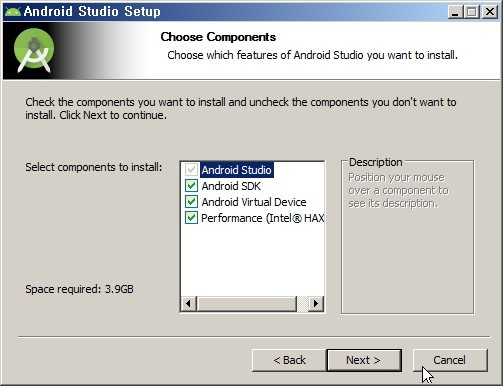
\includegraphics[width=80mm,scale=1.3]{android3}
\end{center}

\begin{center}
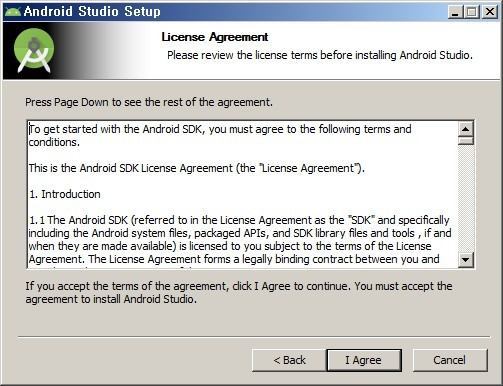
\includegraphics[width=80mm,scale=1.3]{android4}
\end{center}

\begin{center}
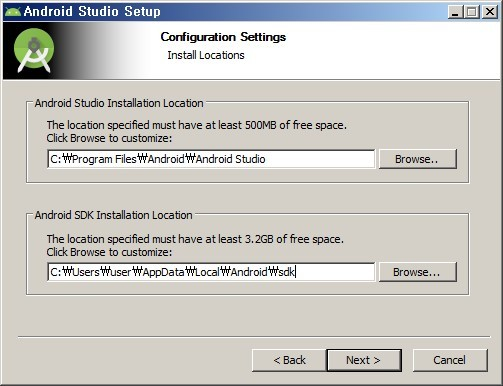
\includegraphics[width=80mm,scale=1.3]{android5}
\end{center}

\begin{center}
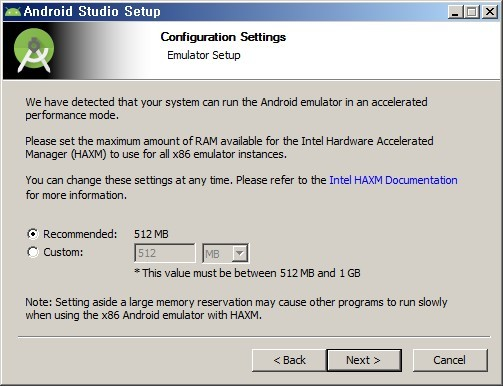
\includegraphics[width=80mm,scale=1.3]{android6}
\end{center}

\begin{center}
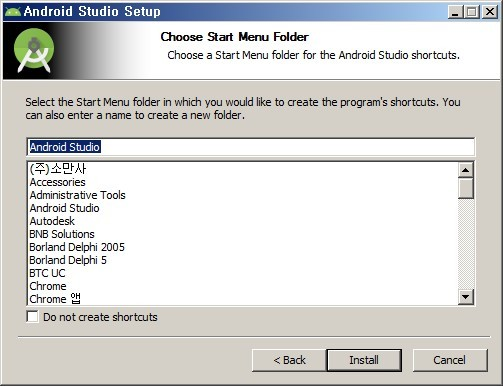
\includegraphics[width=80mm,scale=1.3]{android7}
\end{center}

\begin{center}
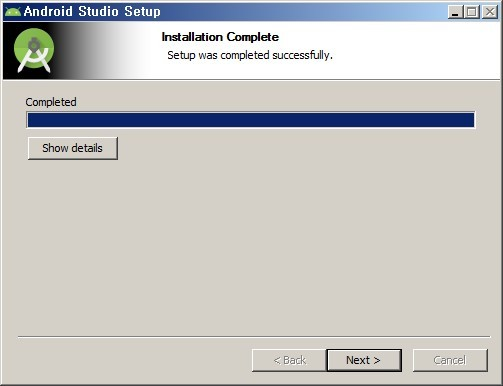
\includegraphics[width=80mm,scale=1.3]{android8}
\end{center}

\begin{center}
Select the UI theme\\ [1\baselineskip]
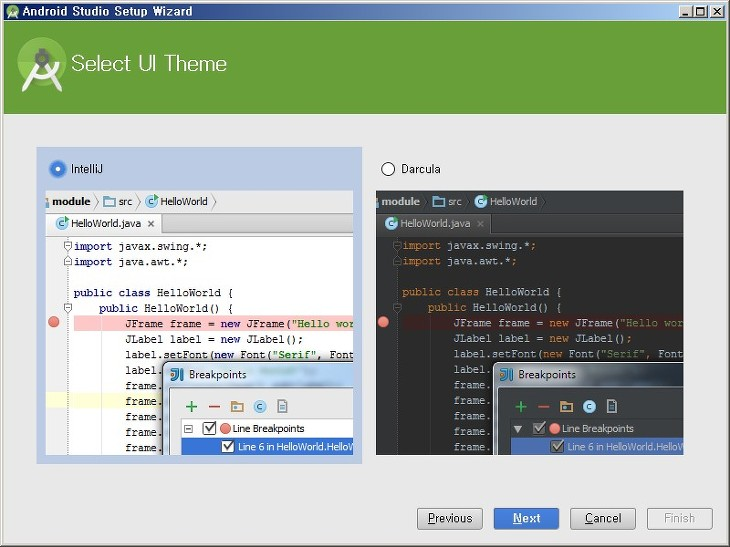
\includegraphics[width=80mm,scale=1.3]{android9}
\end{center}

\begin{center}
Initial menu screen\\ [1\baselineskip]
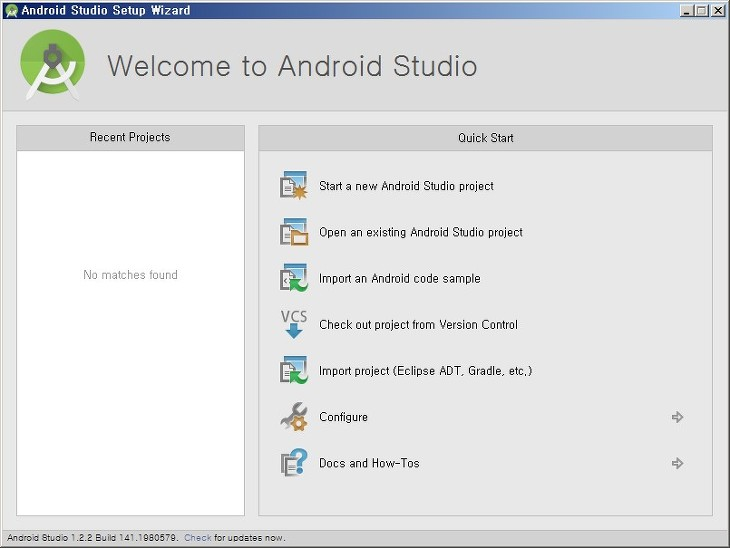
\includegraphics[width=80mm,scale=1.3]{android10}
\end{center}
\newpage
\begin{center}
Press configure and install SDK in android SDK manager\\ [1\baselineskip]
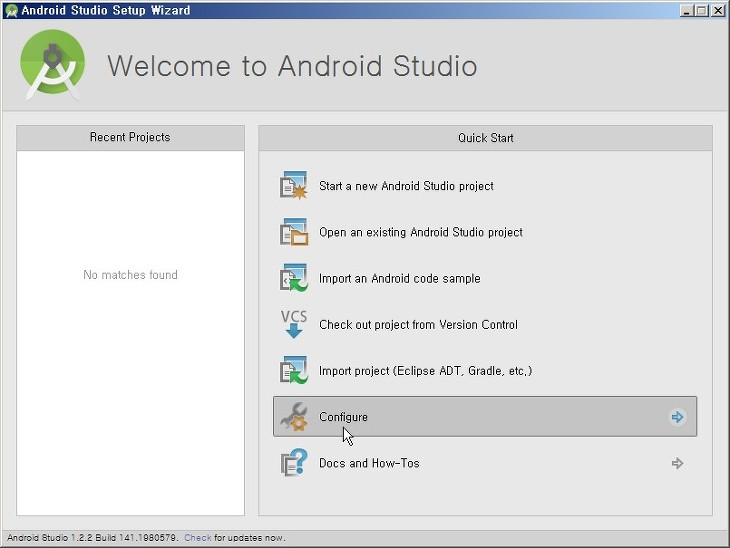
\includegraphics[width=80mm,scale=1.3]{android11}
\end{center}

\begin{center}
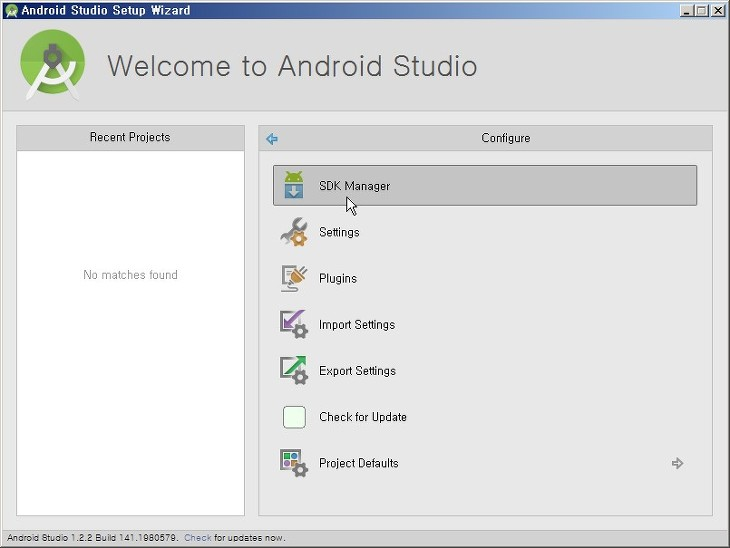
\includegraphics[width=80mm,scale=1.3]{android12}
\end{center}

\begin{center}
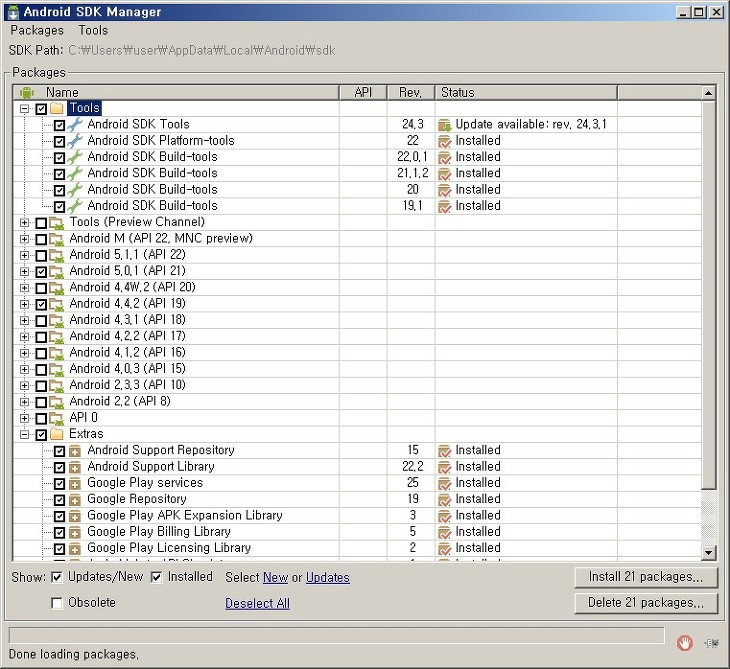
\includegraphics[width=80mm,scale=1.3]{android13}
\end{center}
\newpage
\begin{center}
Make your own project\\ [1\baselineskip]
\includegraphics[width=80mm,scale=1.3]{android14}
\end{center}

\subsection{Install Chrome}
\begin{center}
Go to https://www.google.com/intl/ko/chrome/browser/features.html and download the file\\
From now on, in every steps, remain basic setting and just follow until finish\\ [1\baselineskip]
\includegraphics[width=80mm,scale=1.3]{chrome1}
\end{center}

\begin{center}
\includegraphics[width=80mm,scale=1.3]{chrome2}
\end{center}

\begin{center}
\includegraphics[width=80mm,scale=1.3]{chrome3}
\end{center}

\begin{center}
\includegraphics[width=80mm,scale=1.3]{chrome4}
\end{center}


\subsection{Install Java JDK}
\begin{center}
Go to Oracle site and choose 'Downloads-Java SE'\\ [1\baselineskip]
\includegraphics[width=80mm,scale=1.3]{jdk1}
\end{center}

\begin{center}
\includegraphics[width=80mm,scale=1.3]{jdk2}
\end{center}
\newpage
\begin{center}
Accept license agreement and choose which fits with your windows version\\ [1\baselineskip]
\includegraphics[width=80mm,scale=1.3]{jdk3}
\end{center}

\begin{center}
After the downloads, go to control panel, set path and environment variables\\ [1\baselineskip]
\includegraphics[width=80mm,scale=1.3]{jdk4}
\end{center}
\newpage
\begin{center}
Select the user variable which is at the top\\ [1\baselineskip]
\includegraphics[width=80mm,scale=1.3]{jdk5}
\end{center}

\begin{center}
Click creation, set your directory folder and confirm\\ [1\baselineskip]
\includegraphics[width=80mm,scale=1.3]{jdk6}
\end{center}

\begin{center}
Click the user variable, click edit button, and modify path variable\\ [1\baselineskip]
\includegraphics[width=80mm,scale=1.3]{jdk7}
\end{center}

\begin{center}
Confirm through command that the installation is correctly done\\ [1\baselineskip]
\includegraphics[width=80mm,scale=1.3]{jdk8}
\end{center}

\newpage

\section{Discussion}
Because we used first Amazon EC2, we had a difficulty understanding to handle EC2 instance and overall flow. Also, at EC2 instance, we had a difficulty installing web server. Furthermore, to use WebRTC API, SSL was required and https protocol is required. In the process, we spent too much time looking up ways to install SSL into EC2 server because many bug and error emerged in the process. Also, the information about installing SSL was insufficient. From this, we learned many security policy for web. In addition, also it was almost first time, it was difficult to build overall web development environment for function of streaming.\\

At first. we want to use JAVA. But JAVA is hard to develop WebView. So We change our programming language to C-Sharp however, we never use the C-Sharp before. So we had hard time to get used to C-Sharp. And we want to use the Chrome WebView but C-sharp’s WebView is based on Explorer. So We had hard time to find the library that use the WebView based Chrome. Finally, we found the Dotnet Api. So We can use the WebView based Chrme at C-Sharp. And Android also don’t use the WebView based Chrome. So again, We had hard time to find the library that use the WebView based Chrome in android. Again, We found the ChromView module. But we never used Android Module before, It was very hard to set up module to our project. But we made it. \\

There were lots of difficulties in documentation and using paper making program, latex. Documentation style was first seen, especially latex was first using program. So we could use this after the long-time study. Also, documenting in latex, there were many cases of errors which is caused by tiny mistakes. That kinds of errors were very difficult to realize and inserting various types of tables and pictures because we didn't know about correct commands. So we invested pretty much time in finding latex directions. There was nothing about communication problem in our team. We met two or three days every weeks and discussed about project and researched. Although we failed to implement streaming using java, it was already enough beneficial time for us. It was hard time using Amazon EC2 and changing process of java to C-Sharp, we think these kinds of trial and error also can be the experience. Lastly, we didn't feel the need of using Github because we always meet and do the tasks together.\\

\end{document}





